
\documentclass[a4paper,10pt]{article}

%%% ---------------- %%%
% LaTeX heeft een zekere basisfunctionaliteit maar meestal is deze onvoldoende. Daarvoor bestaan er bijkomende pakketten.
%
% P.S. In een regel is alles na '%' een opmerking. Deze worden niet opgenomen bij compilatie van het document.
%%% ---------------- %%%

\usepackage[english]{babel}   % Spellingcorrectie en titels in NL
\usepackage{graphicx}       % Pakket voor afbeeldingen
\usepackage[colorlinks, linkcolor=black, citecolor=black, urlcolor=black]{hyperref}
\usepackage{geometry}       % Pakket voor pagina-indeling
\geometry{tmargin=3cm, bmargin=2.2cm, lmargin=2.2cm, rmargin=2cm}
\usepackage{todonotes}      % Pakket voor figuur 'placeholders'
\usepackage{subcaption}
\usepackage{ifthen}
\usepackage{enumitem}
\usepackage{amsmath}        % Pakket voor vergelijkingen
\usepackage{floatrow}
\usepackage{amsmath, amssymb, amsthm}
\usepackage{listings}
\usepackage{xcolor}
\usepackage{siunitx}
\usepackage{hhline}
\definecolor{backcolour}{rgb}{0.95,0.95,0.92}
\lstdefinestyle{mystyle}{backgroundcolor=\color{backcolour},  language=Matlab }
\lstset{style=mystyle}
\floatsetup[table]{capposition=top}     % Pakket dat bovenschriften creëert bij tabellen ipv de standaard onderschriften.
\usepackage{float}
\usepackage{svg}
\usepackage{wasysym}
\usepackage{framed}
\usepackage{lscape}
\usepackage{array}
\usepackage{bold-extra}
\newcommand{\textbox}[2][6]{
\begin{framed}
\noindent#2
\end{framed}}
\usepackage[toc,page]{appendix}

\usepackage{acro}
\acsetup{list/template=tabular, format/short = \scshape}

\DeclareAcronym{os}{
  short={os},
  long=Operating System
}
\DeclareAcronym{mvc}{
  short={mvc},
  long=Model-View-Controller,
}
\DeclareAcronym{orm}{
  short={orm},
  long=Object Relational Mapper,
}
\DeclareAcronym{http}{
  short={http},
  long=HyperText Transport Protocol,
}
\DeclareAcronym{https}{
  short={https},
  long=HyperText Transport Protocol Secure,
}
\DeclareAcronym{html}{
  short={html},
  long=HyperText Markup Language,
}
\DeclareAcronym{ssl}{
  short={ssl},
  long=Secure Socket Layer,
}
\DeclareAcronym{tls}{
  short={tls},
  long=Transport Layer Security,
}
\DeclareAcronym{wsgi}{
  short={wsgi},
  long=Web Server Gateway Interface,
}
\DeclareAcronym{vpn}{
  short={vpn},
  long=Virtual Private Network,
}
\DeclareAcronym{rest}{
  short={rest},
  long=Representational State Transfer,
}
\DeclareAcronym{api}{
  short={api},
  long=Application Programming Interface,
}
\DeclareAcronym{json}{
  short={json},
  long=JavaScript Object Notation,
}
\DeclareAcronym{anpr}{
  short={anpr},
  long=Automatic Number Plate Recognition,
}
\DeclareAcronym{udms}{
  short={udms},
  long=Ultrasonic Distance Measuring Sensor,
}
\DeclareAcronym{iot}{
  short={IoT},
  long=Internet of Things,
}
\DeclareAcronym{mp}{
  short={mp},
  long=Mega Pixel,
}
\DeclareAcronym{cpu}{
short={cpu},
long=Central Processing Unit,
}
\DeclareAcronym{ram}{
short={ram},
long=Random Access Memory
}
\DeclareAcronym{sql}{
short={sql},
long=Structured Query Language
}
\DeclareAcronym{rdbms}{
short={rdbms},
long=Relational Database Management System 
}
\DeclareAcronym{ocr}{
short={ocr},
long=Optical Character Recognition
}
\DeclareAcronym{gdpr}{
short=gdpr,
long=General Data Protection Regulation
}
\DeclareAcronym{js}{
short=js,
long=JavaScript
}
\DeclareAcronym{lan}{
short=lan,
long=Local Area Network
}
\DeclareAcronym{gui}{
short=gui,
long=Graphical User Interface
}
\DeclareAcronym{ips}{
short=ips,
long=Intelligent Parking System
}
\DeclareAcronym{ddos}{
short=ddos,
long=Distributed Denial of Server
}
\DeclareAcronym{csrf}{
short=csrf,
long=Cross Site Request Forgery
}
\DeclareAcronym{idor}{
short=idor,
long=Indirect Object Reference
}
\DeclareAcronym{lcd}{
short=lcd,
long=Liquid Crystal Display
}
\DeclareAcronym{2fa}{
short=2fa,
long=Two Factor Authentication
}
\DeclareAcronym{rce}{
short=rce,
long=Remote Code Execution
}
\DeclareAcronym{xss}{
short=xss,
long=Cross Site Scripting
}
\DeclareAcronym{acl}{
short=acl,
long=Access Control Level
}
\DeclareAcronym{ssrf}{
short=ssrf,
long=Server-Side Request Forgery
}
\DeclareAcronym{jwt}{
short=jwt,
long=\textsc{json} Web Tokens
}
\DeclareAcronym{totp}{
short=totp,
long=Timed One Time Password
}
\DeclareAcronym{led}{
short=led,
long= Light Emitting Diode
}
\DeclareAcronym{mdf}{
short=mdf,
long= Medium Density Fibreboard
}
\DeclareAcronym{url}{
short=url,
long= Uniform Resource Locator
}
\DeclareAcronym{wifi}{
short=WiFi,
long= Wireless Fidelity,
short-format = \rmfamily ,
}
\DeclareAcronym{apm}{
short=apm,
long= Application Performance Monitoring,
}
\DeclareAcronym{cvc}{
short=cvc,
long= Card Validation Code,
}
\DeclareAcronym{qr}{
short=qr,
long= Quick Response,
}
\DeclareAcronym{acm}{
short=acm,
long= Access Control Misconfiguration,
}
\DeclareAcronym{mitm}{
short=mitm,
long= Man In The Middle,
}
\DeclareAcronym{tpa}{
short=tpa,
long= Third-Party Authenticator,
}
\DeclareAcronym{cdn}{
short=cdn,
long= Content Delivery Network,
}

\DeclareAcronym{dos}{
short=dos,
long= Denial of Service,
}

\usepackage{tocloft}

\newlength{\mylen}
\setlength{\mylen}{5px}

\renewcommand{\cftfigpresnum}{\figurename\enspace}
\renewcommand{\cftfigaftersnum}{:}
\settowidth{\mylen}{\cftfigpresnum\cftfigaftersnum}
\renewcommand{\cftsecleader}{\cftdotfill{\cftdotsep}}
\addtolength{\cftfignumwidth}{25px}

\renewcommand{\cfttabpresnum}{\tablename\enspace}
\renewcommand{\cfttabaftersnum}{:}
\settowidth{\mylen}{\cfttabpresnum\cfttabaftersnum}
\renewcommand{\cftsecleader}{\cftdotfill{\cftdotsep}}
\addtolength{\cfttabnumwidth}{25px}
\newcommand{\tabitem}{~~\llap{\textbullet}~~}

\setlength\parindent{1em}
\newcommand{\ind}{\hspace{1.2em}}

\usepackage{titlesec}

\setcounter{secnumdepth}{4}

\titleformat{\paragraph}
{\normalfont\normalsize\bfseries}{\theparagraph}{1em}{}
\titlespacing*{\paragraph}
{0pt}{3.25ex plus 1ex minus .2ex}{1.5ex plus .2ex}


\begin{document}
\begin{titlepage}
    \newpage
    \pagenumbering{Roman}
    \thispagestyle{empty}
    \frenchspacing
    \hspace{-0.2cm}
    \hspace{0.2cm}
    \hspace{0.2cm}
    
\includegraphics[height=2.5cm]{images/logoFirW.jpg}
    \hspace{5.8cm}
    
\includegraphics[height=2.5cm]{images/kul_logo.jpg}
    %\begin{minipage}[b]{8cm}
        %\Large{Katholieke\newline Universiteit\newline Leuven}\smallskip\newline
        %\large{}\smallskip\newline
        %\textbf{Faculteit\newline Ingenieurswetenschappen}\smallskip
    %\end{minipage}
    \hspace{\stretch{1}}
    \vfill
    \vspace{0.5cm}
    \centering\Large{\rm\textbf{{Problem Solving and Engineering Design part 3}}}
    \vspace*{0.5cm}\vfill
    \begin{center}
        \begin{minipage}[t]{\textwidth}
            \begin{center}
                \Large{\rm{\textbf{CW1B2}}}\\
                \vspace{0.3cm}
                \normalsize{\rm {Ruben Mariën (r0883561)}}\\
                {\rm {Robin Martens (r0885874)}}\\
                {\rm {Neel Van Den Brande (r0876234)}}\\
                {\rm {Rik Vanhees (r0885864)}}\\
                {\rm {Rune Verachtert (r0884615)}}\\
                {\rm {Tuur Vernieuwe (r0886802)}}\\
                \vspace{2.5cm}
                
                \Huge{\rm\textbf{An intelligent parking garage}} \\
                \vspace{1cm}
                \large{\rm\textsc{{preliminary report}}} \\
                \vspace{4cm}
                {\rm \large\underline{Co-titular}} \\
                {\rm \normalsize{prof. dr. ir. Bart De Decker}} \\
                \vspace{0.5cm}
                {\rm \large\underline{Coaches}} \\
                {\rm \normalsize{Shuaibu Musa Adam}} \\
                {\rm \normalsize{Shirin Kalantari}} \\
                {\rm \normalsize{Hamdi Trimech}} \\
                \vspace{1.5cm}
                \LARGE{\rm\textsc{academic year 2022-2023}}
                \vfill
            \end{center}
        \end{minipage}
    \end{center}
    \vfill
\end{titlepage}

\vspace*{\fill} % for vertical centering 1/3

\textbox{
\begin{center}
    \textit{\textbf{Declaration of originality}}
\end{center}

\noindent \textit{We hereby declare that this submitted draft is entirely our own, subject to feedback and support given us by the didactic team, and subject to lawful cooperation which was agreed with the same didactic team.}
\textit{Regarding this draft, we also declare that:}

\begin{enumerate}
    \item \textit{Note has been taken of the text on academic integrity (\url{https://eng.kuleuven.be/studeren/masterproef-en-papers/documenten/20161221-academischeintegriteit-okt2016.pdf}).}
    \item \textit{No plagiarism has been committed as described on \url{https://eng.kuleuven.be/studeren/masterproef-en-papers/plagiaat}.}
    \item \textit{All experiments, tests, measurements, …, have been performed as described in this draft, and no data or measurement results have been manipulated.}
    \item \textit{All sources employed in this draft – including internet sources – have been correctly referenced.}
\end{enumerate}

\noindent \textit{This we solemnly declare, in our own free will and on our own word of honor.} 
}
\vspace*{\fill}
\vspace{\baselineskip}


\newpage

\addcontentsline{toc}{section}{Contents}
\tableofcontents
\clearpage

\addcontentsline{toc}{section}{\listfigurename}
\listoffigures

\clearpage
\addcontentsline{toc}{section}{\listtablename}
\listoftables

\clearpage
\addcontentsline{toc}{section}{List of Acronyms}
\acsetup{format/short=\MakeUppercase}
\printacronyms[name=List of Abbreviations]
\acsetup{format/short=\scshape}

\newpage

\pagenumbering{arabic}
\setcounter{page}{1}
\newpage


\section{Introduction}\label{Introduction}

% Brede context + versmalling
People these days value efficiency in life on all fronts ever higher. Time has become more and more valuable and loss of time has to be minimal. Since almost every family owns a car with most of them even owning two or three \cite{vehicles_in_families}, and travelling by car has become increasingly popular. Parking efficiency is an element that affects everyone on a near daily basis. This requires engineers to invent and examine new solutions to improve this parking experience. The dissatisfaction with the classic ticket system in most parking garages, causes an evolution into more digital and automated systems. Often accomplished through licence plate recognition in combination with mobile apps and automated payment options \cite{4411}. Despite the convenience of these systems, it poses a risk of a privacy breach \cite{privacy_breach}. Therefore, sufficient attention should be given to the security of these systems. The privacy of the user is the number one priority.\\

% Doel
The main goal of the project is to make an automatic parking garage using \ac{iot} devices. This means that a client will be able to drive into the garage and park his/her car here for a certain duration of time. Then, drive away without having to pay with the use of a ticket. This is accomplished by cameras and \ac{anpr} software, together with a mobile application. \\

This intermediate report will describe both the mechanical and software aspects of the current state of the design. Section \ref{sec:Problem description} describes the working of the entire system in an abstract way. Section \ref{sec:implementation} gives the concrete implementation of the system. The reasons why the components of the system were chosen can be found in section \ref{sec:design-motivation}.Then, section \ref{sec:case-example} will describe a sample user experience in the \ac{ips}. Section \ref{sec:coclusion} will give a conclusion of the project and finally, section \ref{sec:course-integration} gives an overview of the course integration with the different courses in the first and second year of the Bachelor in Engineering Science.

%Section \ref{sec:mechanical-design} describes the final mechanical design of the parking garage, the considered design alternatives and the motivation for the current design. The software design is described in Section \ref{sec:software-design}. It is broken down into three parts, which represent the three main components of the \ac{ips}: the Raspberry Pi software, the frontend application and the backend. Then, Section \ref{sec:user-experience} will describe a sample user experience in the \ac{ips}. Sections \ref{sec:budget} and \ref{sec:planning} describe practical aspects of the course of the project, namely the budget and the planning respectively. Finally, Section \ref{sec:course-integration} gives an overview of the course integration with the different courses in the first and second year of the Bachelor in Engineering Science.

\subsection{Problem description}\label{sec:Problem description}
% Describe the problem shortly and states which features are invaluable in the parking garage.
The official problem description is very broad: ``design a fully functional intelligent parking garage'' with the following requirements \cite{project_description}:
\begin{enumerate}
    \item the parking garage detects the amount of available parking lots;
    \item the amount of available parking lots is displayed across multiple screens;
    \item drivers can reserve a parking lot;
    \item the parking garage detects entering and exiting vehicles which eliminates the need of parking tickets.
\end{enumerate}
Therefore, the following infrastructure has to be designed, provided and built:
\begin{enumerate}
    \item sensors to detect the occupancy of a parking lot;
    \item a central server which stores and provides all the necessary data;
    \item a frontend application which the clients can use.
\end{enumerate}
The main research question this project tries to answer is ``\textit{How can we realise a safe \ac{iot} -infrastructure which makes parking easier, faster and foremost, safer?}'' \cite{project_description}.

\clearpage
\section{General design description}
% Provide an abstract overview of the entire system, integrating both the hardware and the software parts.
This section describes the entire working of the system in an abstract way. The details of the concrete implementation can be found in Section \ref{sec:implementation}.

\ind The \ac{ips} consists of three main parts: the on site sensors and gateway, the frontend application and the backend. \\

The backend is the central entity in the system, as both the local system and the frontend application connect to it in order to query data. This is done via a \ac{rest} \ac{api}, which transfers data in \ac{json}-format; the standard for \ac{rest} \ac{api}s \cite{rest_apis}. The backend consists out of the combination of the servers which handles the incoming requests and the database, which stores all the information about the parking garage (e.g. occupancy of parking lots, users inside the parking garage, etc.).
The backend also hosts the web variant of the frontend application and thus needs proper redirecting in order to redirect requests to the right destinations (in casu the frontend application or the database). The backend resides in a separate location (e.g. a data centre), separated from the actual garage. \\

The local setup requires a gateway  (\ac{iot}-device) and sensors installed in the physical garage. The sensors and the gateway are preferably connected through a \ac{lan}, but cable wiring is also possible, although less practical.

\ind The gateway is a micro-controller or \ac{iot}-device which is the central processing unit for the local system. It can post and request data from the backend and controls the interaction between the different sensors. It performs only simple logic tasks and delegates from complex calculation to the backend.

\ind Two cameras detect the cars which are entering or exiting the parking garage, via \ac{anpr}. They are linked via the gateway with two servo motors, which control the barriers for entering and exiting the garage. Inside the garage, sensors detect if a parking lot is occupied or not. A \textsc{led} visually indicates to the drivers if the parking lot is occupied. Furthermore, a display indicates the amount of free spots left in the garage. \\

The frontend application serves as a \ac{gui} for the user to interact with the backend database. The application comes in two formats: a mobile application which is installable on both iOS and Android and a web application in the form of a website. Both variants have the same functionality.

\begin{figure}[htp]
    \centering
    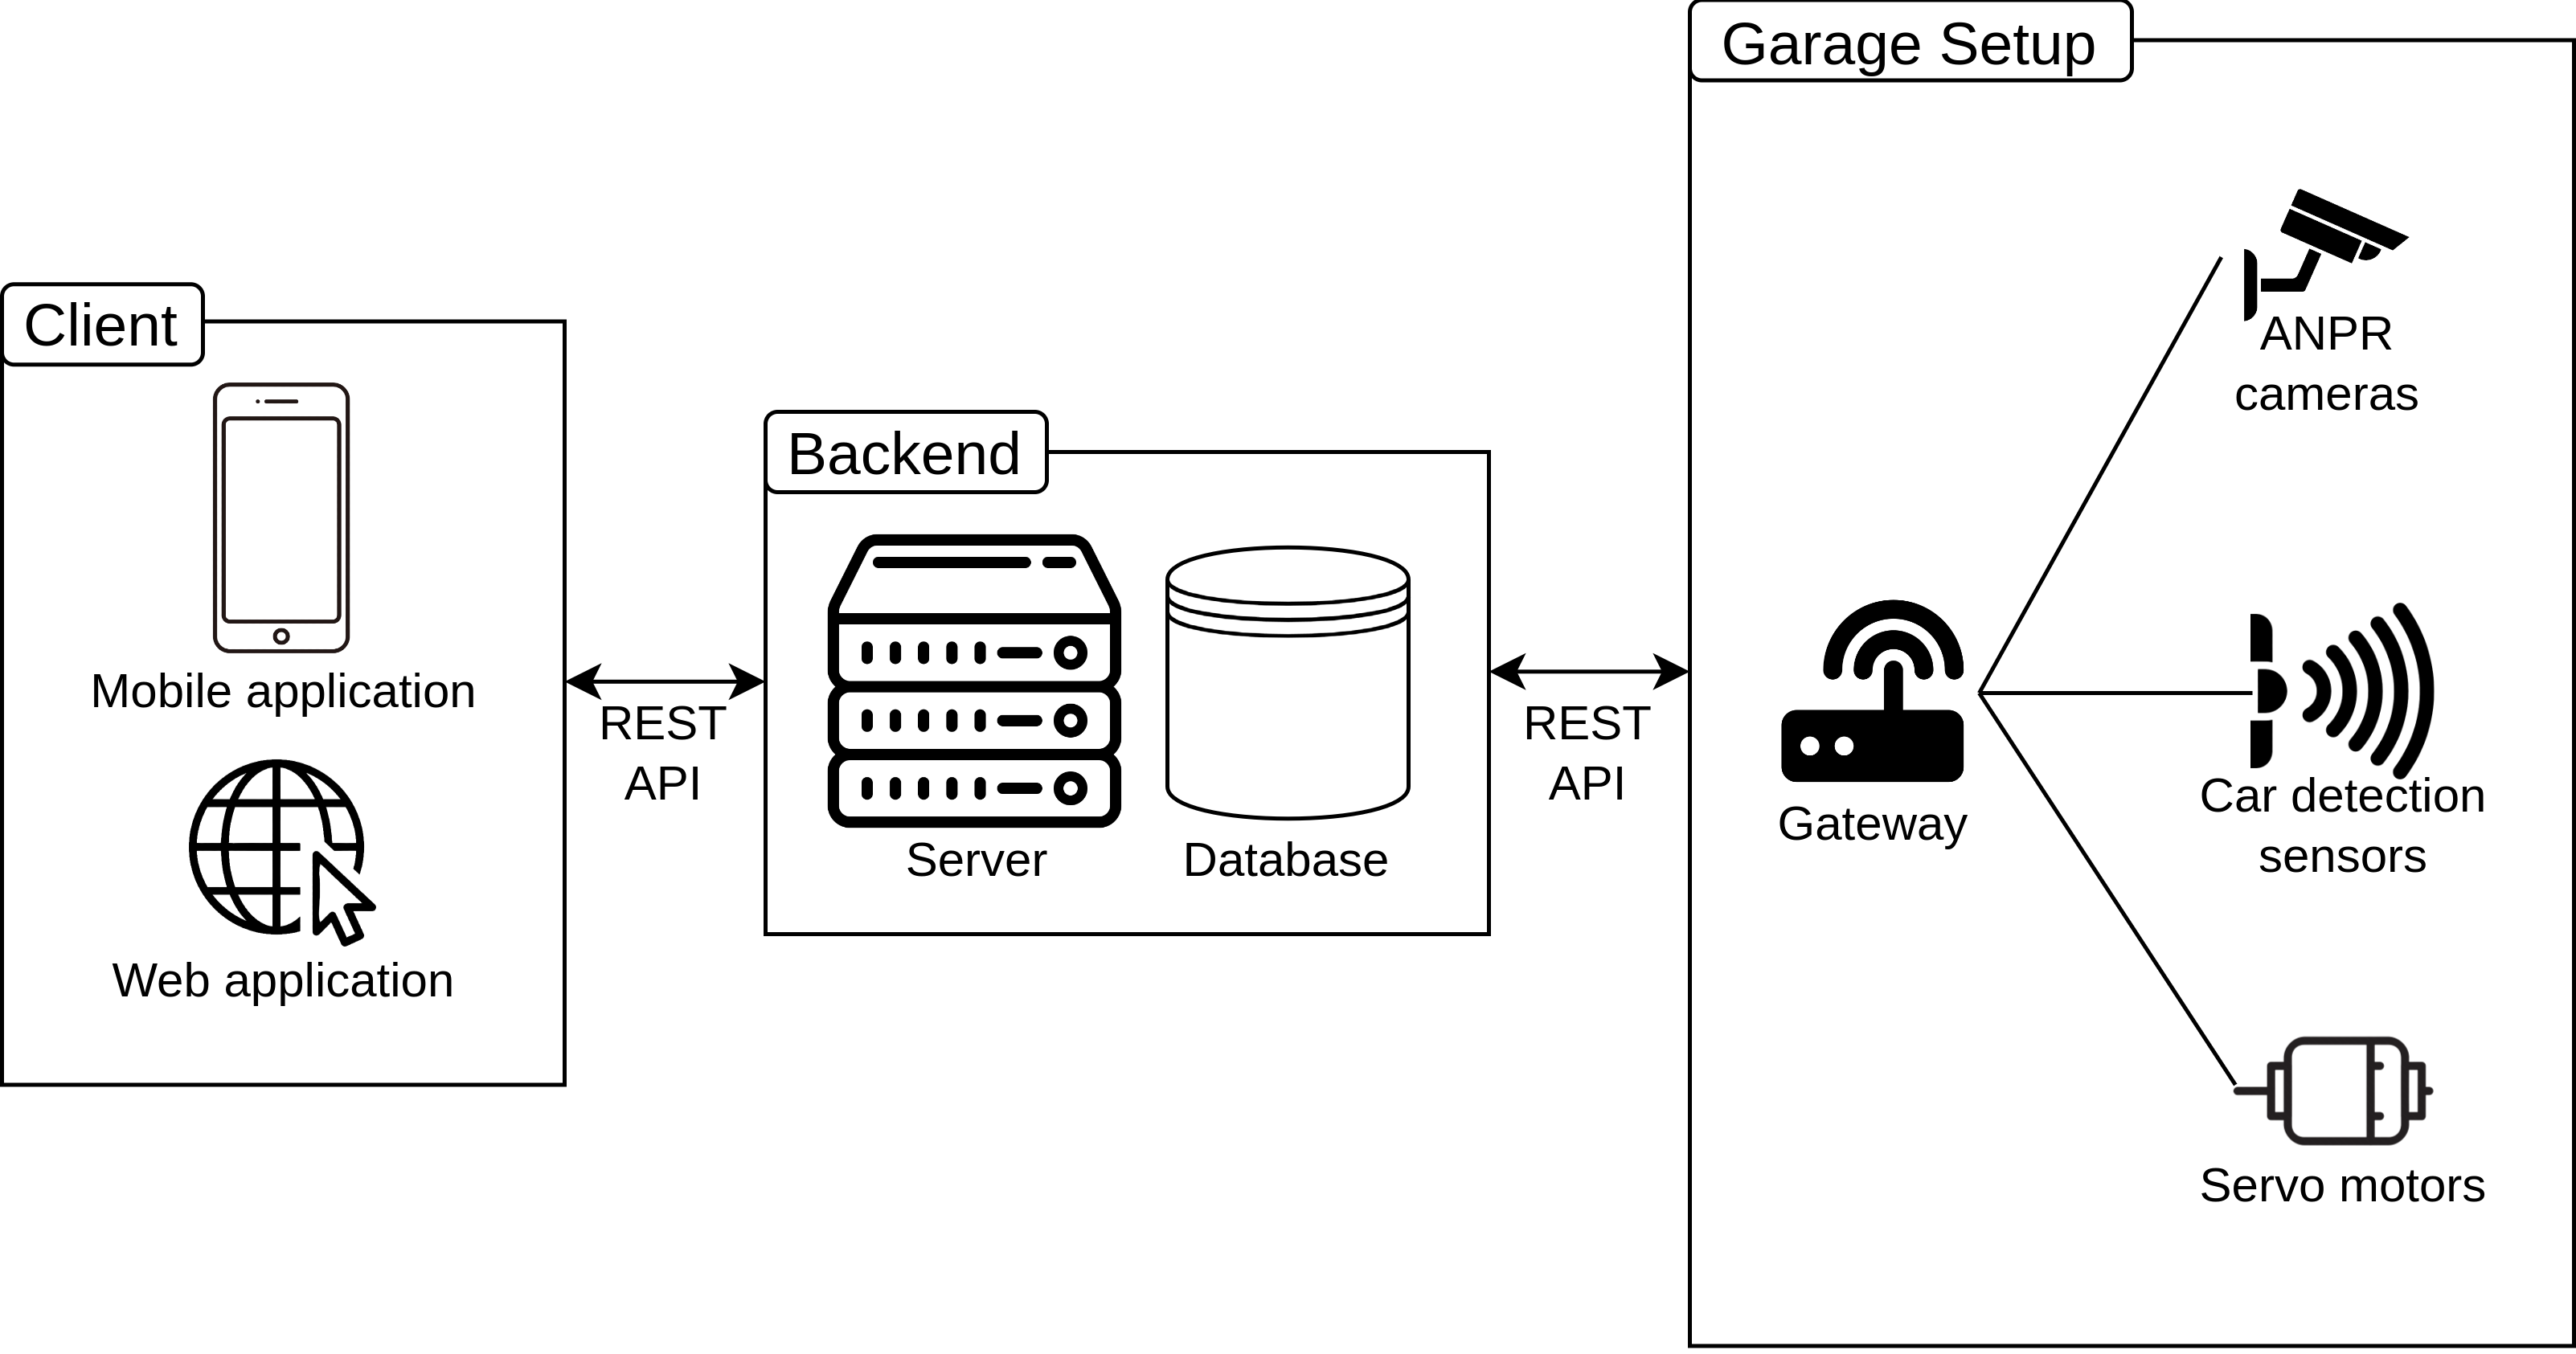
\includegraphics[width=12cm]{images/abstract_diagram.drawio.png}
    \caption[Abstract overview of the intelligent parking system.]{Abstract overview of the intelligent parking system. The backend can be deployed on one psychical machine, which can run the proxy server and the database server in parallel.}
    \label{fig:my_label}
\end{figure}


\subsection{Core functionalities}\label{sec:core-functionalities}
The three main spearheads of the \ac{ips} described above are user privacy, security and ease of use. Table \ref{tab:core-functionalities} gives a summary of this paragraph, listing the three core functionalities, together with the steps taken to achieve them.\\ 

The ease of use is split up in three sub-objectives.

\ind Firstly, it is not necessary for users of the parking garage to install the mobile application or even to have a pre-existing account. It possible that users can drive to the parking garage and park without any need for prior setup, but with an almost equal user experience.

\ind Secondly, if the user creates an account, he/she is able to reserve parking lots in a specific garage from and to specific hours, such that the availability of a free parking lot is guaranteed at arrival of the user.

\ind Thirdly, the infrastructure supports automatic and non-automatic payments from within the frontend application, the former for user which created an account, the latter as an alternative for users without an account. 

\ind Besides the ease of use of a person parking in the garage, the frontend application also supports admin features for a garage owner. A garage owner can add and delete garages from the system, as well as configure the parking lots in a garage. \\

Maximum user privacy is achieved by, firstly, not storing any information that is not needed for operation of the \ac{ips} (least to know principle) and secondly, hashing all user-identifiable and/or sensitive information (e.g. passwords, licence plates, email addresses) before it is stored inside the database. This way, even if an attacker obtains the database, he/she will not be able to retrieve any useful information from it.

\ind The two ways parking in the garage (i.e. with or without a pre-existing account) provide two levels of user privacy. If the user decides to park without an account, no user-identifiable information is stored in the database, except the licence plate, which is deleted upon exit of the garage. This way, it is not possible to retrieve any personal information, nor information about the user's whereabouts from the system. From the standpoint of the system, that user ceases to exist upon exit of the garage. In the other case, license plate information is coupled with the user's email address and a real first and last name, but history of the user's whereabouts are not stored (they are deleted upon exit of the garage).

\ind Making an automatic payment requires payment information from the user. This information is hashed before it is stored inside the database, but the user can opt for a manual payment, in which case no payment details are stored in the database.

\ind Furthermore, a garage owner is not able to query the users or license plates in its garage, only the amount free parking lots left are displayed. \\ 

Security is the last core functionality. This mainly focuses on securing the backend, because it stores all important user information, but also includes securing the mobile application and the local garage setup, such that the sensors, nor the \ac{anpr}-cameras can be hijacked. 

\ind Firstly, the connections between the frontend and the backend and between the backend and the local garage gateway are encrypted. Secondly, the server only accepts traffic coming from the local garage gateway or the mobile application, which prevents \ac{ddos}- and \ac{csrf}-attacks. Thirdly, users can only query the information regarding their own account (i.e. their personal information and bookings), which prevents \ac{idor}-attacks and fourthly, the \ac{api} can only be queried by authenticated users.

\begin{table}[htp]
    \centering
    \caption{An overview of the core functionalities of the entire system and how this is achieved on an abstract level. }
    \begin{tabular}{|>{\bfseries\centering\arraybackslash}m{1in}|>{\centering\arraybackslash}m{8cm}|}
         \hline
         \textbf{Core functionality} & \textbf{Achieved by}  \\
         \hline
         \hline
         Ease of use & \begin{itemize}[left=0pt]
             \item No obligatory account
             \item Reserving parking lots
             \item Automatic and non-automatic payments
         \end{itemize} \\
         \hline
         User privacy & \begin{itemize}[left=0pt]
             \item Least to know principle
             \item Hashing sensitive user information
         \end{itemize}\\
         \hline
         Security &\begin{itemize}[left=0pt]
             \item Encrypted connections
             \item Request origin validation
             \item Authenticated \ac{api}
         \end{itemize} \\
         \hline
    \end{tabular}
    \label{tab:core-functionalities}
\end{table}

\clearpage

\section{Implementation}\label{sec:implementation}
% Provide a clear explination of the used software, without an explination why we used it (this is explained in the next section).

\subsection{Parking garage}\label{sec:implementation-parking-garage}

\subsection{On site system}\label{sec:implementation-on-site-system}

% Detecting incoming cars

% Detecting parked cars

% 

\subsection{Frontend}\label{sec:implementation-frontend}
This section describes the implementation of the core functionalities of the frontend as described in section \ref{sec:core-functionalities}. The frontend apllication is written in Dart, with the Flutter\footnote{\url{https://flutter.dev/}} framework of Google. Flutter is used, because its main benefits are that it can be runned on any operating system(Android, iOS, MacOS, Linux, Windows, etc.), and it provides type safety and null safety. Further supports flutter a hot reload feature, which makes it easy to develop an application. The next section will give a rough idea how the app will work when you open it.

\subsubsection{First app design}
The first page that users see when they open the app is the login screen, here they will have the option to login with either their existing account or to register a new one. If they choose to make a new account, then the register page pops up. On this page they have to fill in their first name, last name, licence plate, e-mail address and password. These credentials are used to create a secure account for a user that is linked to their licence plate for the automatic payment system. The user is required to confirm the password by entering the same password in another text field. This is required for lowering the chances of accidentally typing the wrong password. Once the necessary text fields are submitted, the user will be able to register their account.

\ind As soon as the account is created, the user can login by hitting the 'Sign in'-button. When that's done, the homepage will pop up and the app will make a request to the backend server to load all the possible garages. While the app is connecting there will be a progress indicator on the screen and the user will still be able to access other buttons like the navigation bar. After all the garages have been loaded into the app, then the user can select one of the garages to make a reseredrvation. Next the reservation screen will pop up of the selected garage. On this screen the user can observe the busiest times of the day and how many spots are left in the garage. If the user is satisfied of this garage, than he/she can book a reservation. There will be the option to choose the time and day and an available spot.

\ind For users who are not familiar with using the app or a mobile app in general, there will be a guide in the navigation bar. Furthermore, the user can see his/her statistics, profile, reservations and adjust their settings. A detailed schematic of the entire app can be found in Appendix \ref{app:app-design} in Figure \ref{fig:AppDesign}. At last there is also an option to sign out of your account. 

\subsubsection{Deployment}
The frontend deployment should support two use cases: users who want to download the mobile application and users who want to access the website. \\

Due to Flutter's nature, it can run natively on all major platforms and operating systems. To make the mobile application accessible to the general public, it should be uploaded to the Google Play Store, the Apple App Store and the Microsoft Store. For the purpose of this project, the application will be installed on the devices of the team members. \\

% We should check if this is even possible to do, otherwise, this is total bogus.
The web application should be hosted on a web server, for the users to be able to access the site. The backend already incorporates a web server, namely Nginx\footnote{\url{https://nginx.org/}}. Apart from being a reverse-proxy for the backend, it also hosts the static files (\textsc{html} and \ac{js}). Figure \ref{fig:deployment-frontend} shows the deployment diagram for the frontend application. Note that the two client devices represent both options of the client of connection to our backend \ac{api}.


\begin{figure}[H]
    \centering
    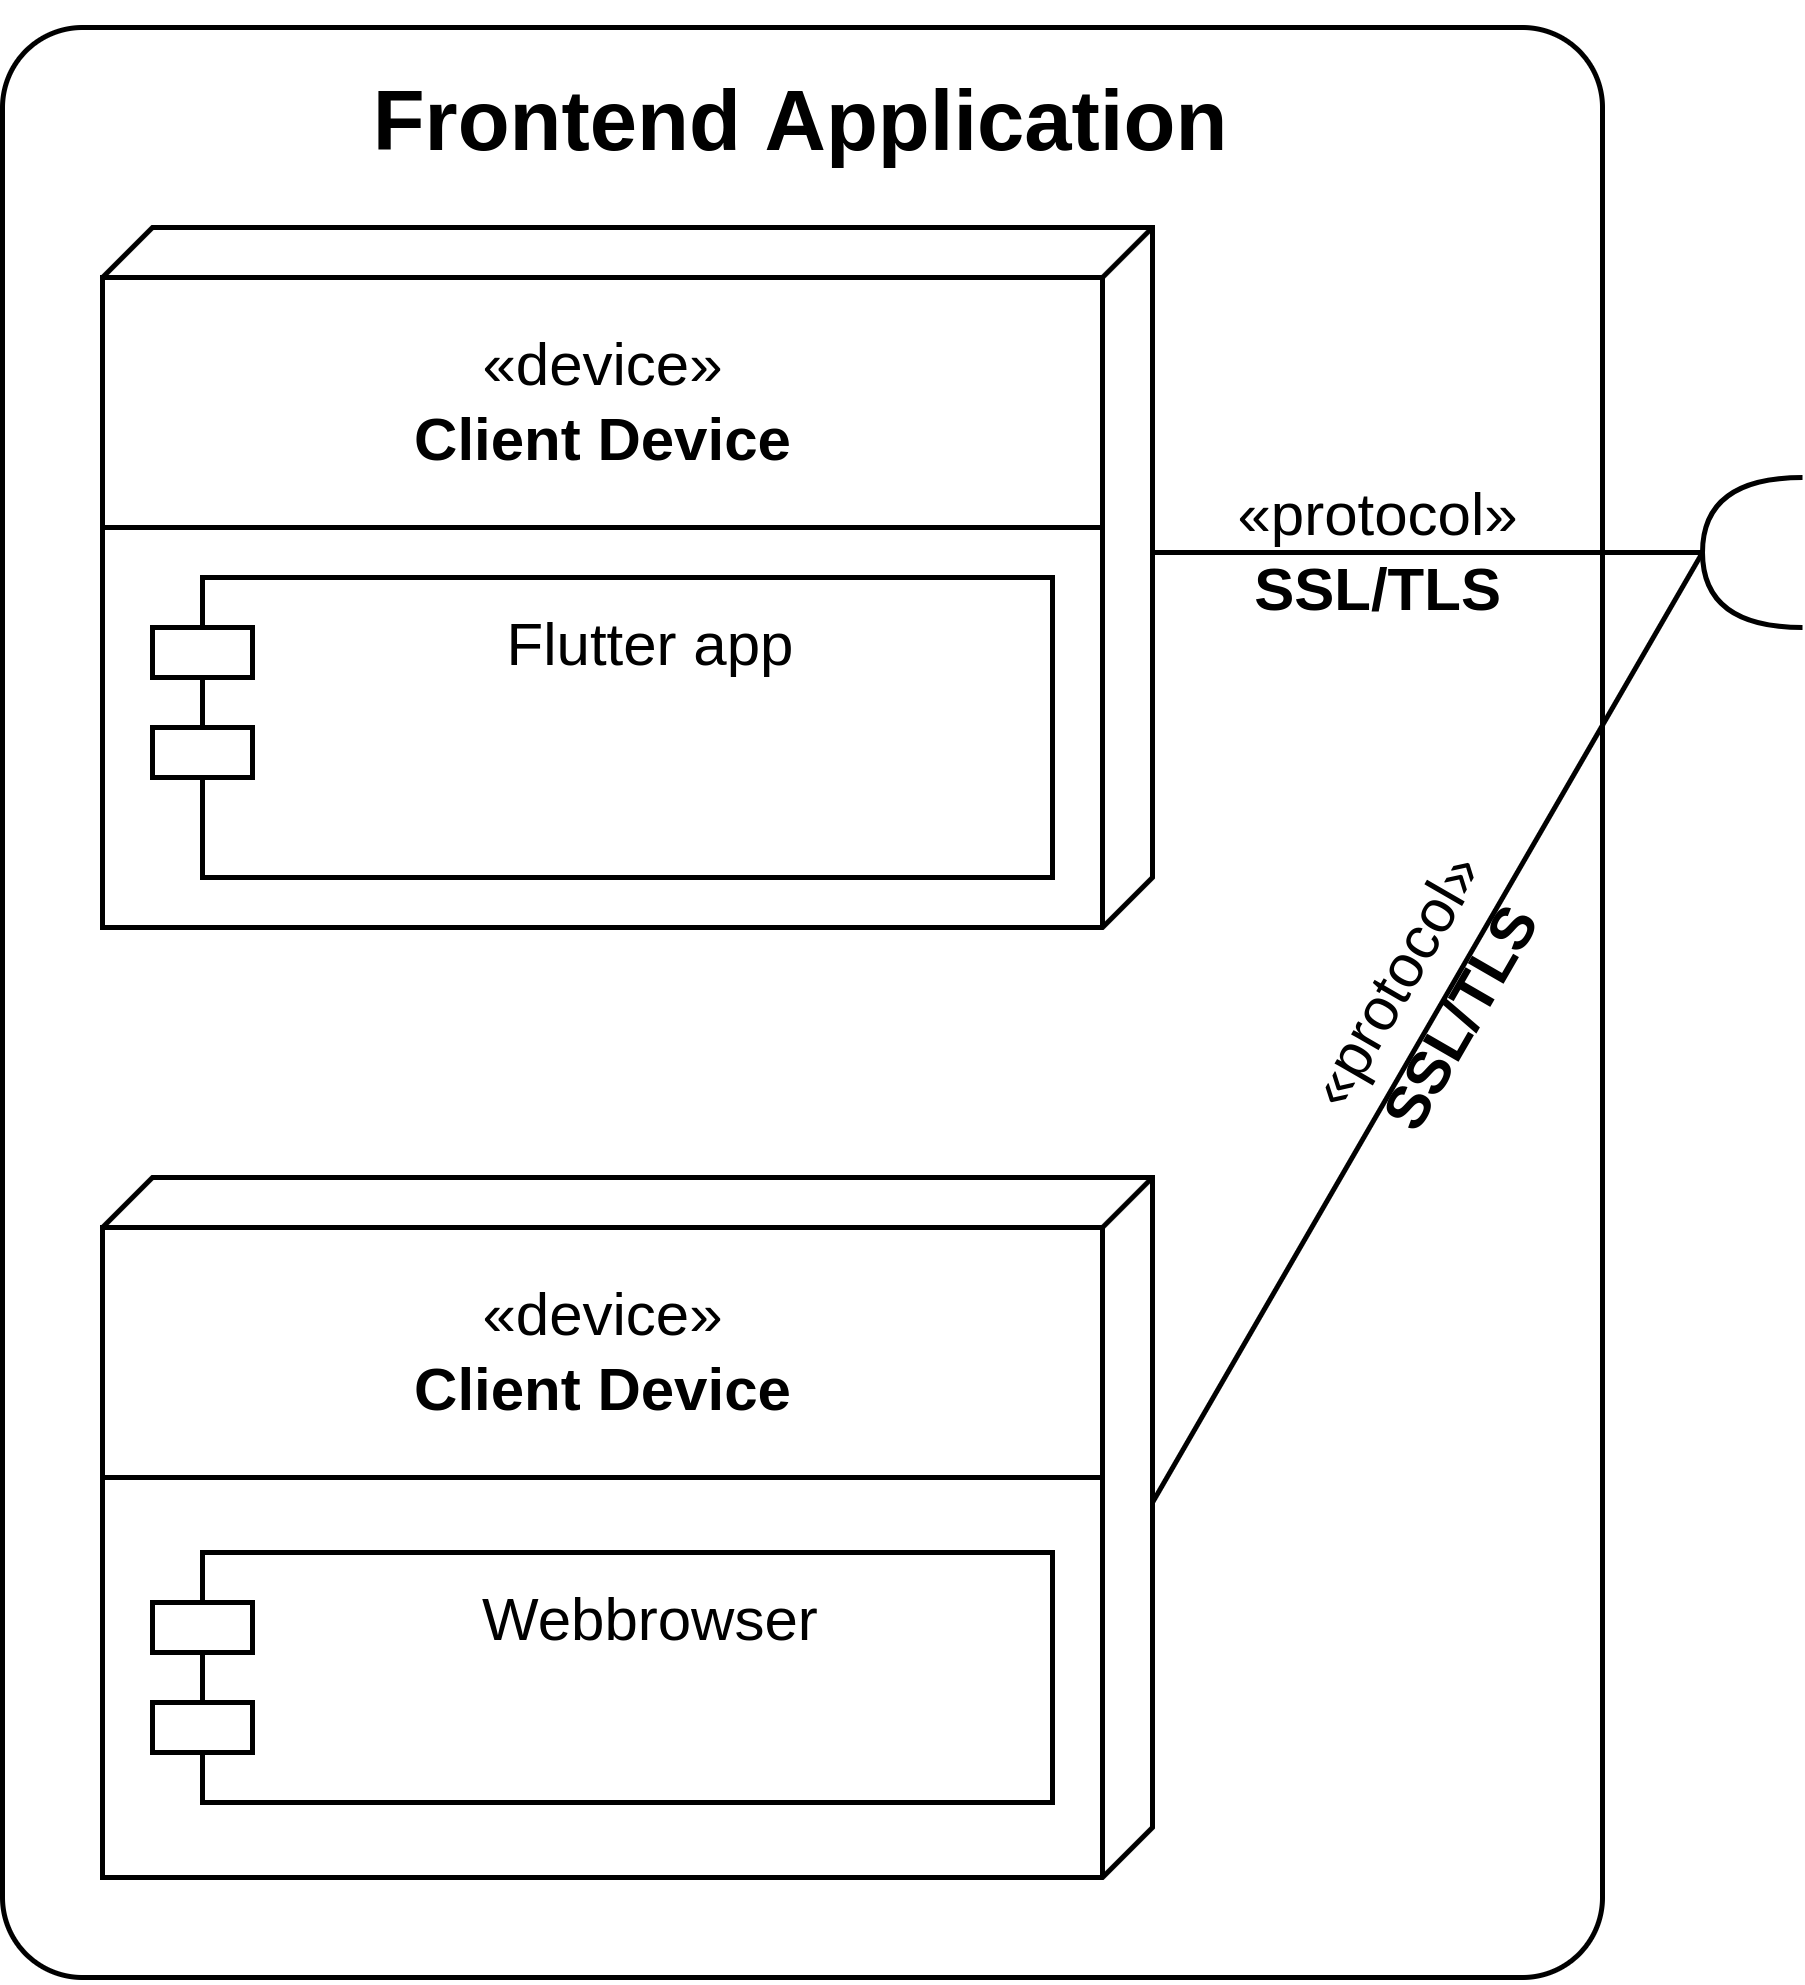
\includegraphics[width=5cm]{images/deployment_diagram_frontend.drawio.png}
    \caption{Deployment diagram of the frontend application.}
    \label{fig:deployment-frontend}
\end{figure}

\clearpage


\subsection{Backend}\label{sec:implementation-backend}
The main functionalities of the backend are described in Section \ref{sec:core-functionalities}. This section describes the implementation of those core functionalities. Section \ref{sec:design-motivation} outlines the augments for the different software used in the backend.

\ind The main parts of the backend described below can run on a single physical machine. The deployment of those services can happen both on a local server or on a cloud server. For the purpose of this project, a local home server is preferred, but in real-world system requires scalability which makes a cloud server indispensable.

\subsubsection{Server}
The server is the main entry point to the outside world of the database and the \ac{rest} \ac{api} and thus needs proper security measures. The encryption of traffic happens on the server, origin validation to prevent \ac{csrf}-attacks is included in the backend application (see Section \ref{sec:backend-application}). 

\ind Nginx is used as the main \ac{http}-server in the backend. It serves as an industry standard for a fast and lightweight server. The most important feature for the backend is that it can handle \ac{ssl}/\ac{tls}-connections and redirect \ac{http}-requests to \ac{https}-requests \cite{nginx}. Furthermore, the server has to redirect incoming requests to the right application, namely, the web variant of the frontend application or the backend application. This is achieved via a \textit{proxy-pass}, which can redirect traffic from one server to another, based on certain conditions in the request (e.g. all \textsc{url}s which start with \texttt{api/} are redirected to the Gunicorn Python server (see below).

\ind Besides a web server, the backend needs a way to communicate between the web server and the actual backend application (in casu the Django application). This is achieved with a \ac{wsgi}. The backend uses Gunicorn\footnote{\url{https://gunicorn.org/}} as its \ac{wsgi}. The main purpose of the \ac{wsgi} is making the deployment more stable and faster. The former is achieved by running multiple instances of the Django application, which improves to overall availability of the system \cite{gunicorn}. Besides improving the deploy stability, the \ac{wsgi} makes it possible to use an Nginx server as reverse proxy for redirecting \ac{http} to \ac{https}-traffic. This is not possible without a \ac{wsgi}.

\ind The services above require a lot of dependencies and configuration files, which can make it tedious to set up on a remote machine. The backend is therefore deployed with Docker containers, which bundles \textit{Docker images} with an \ac{os} in a so-called isolated \textit{container}. This way, all the dependencies are packed inside the container, which eliminates the need of doing a laborious setup on the server machine. In total, there are three containers, one for the Nginx server, one for the Gunicorn gateway which runs the Django application and one for the MySQL database. The containers run as a single service with Docker Compose, which makes communication between the different containers effortless \cite{docker-compose}. Figure \ref{fig:deployment-backend} shows the deployment diagram of the entire backend.

\begin{figure}[htp]
    \centering
    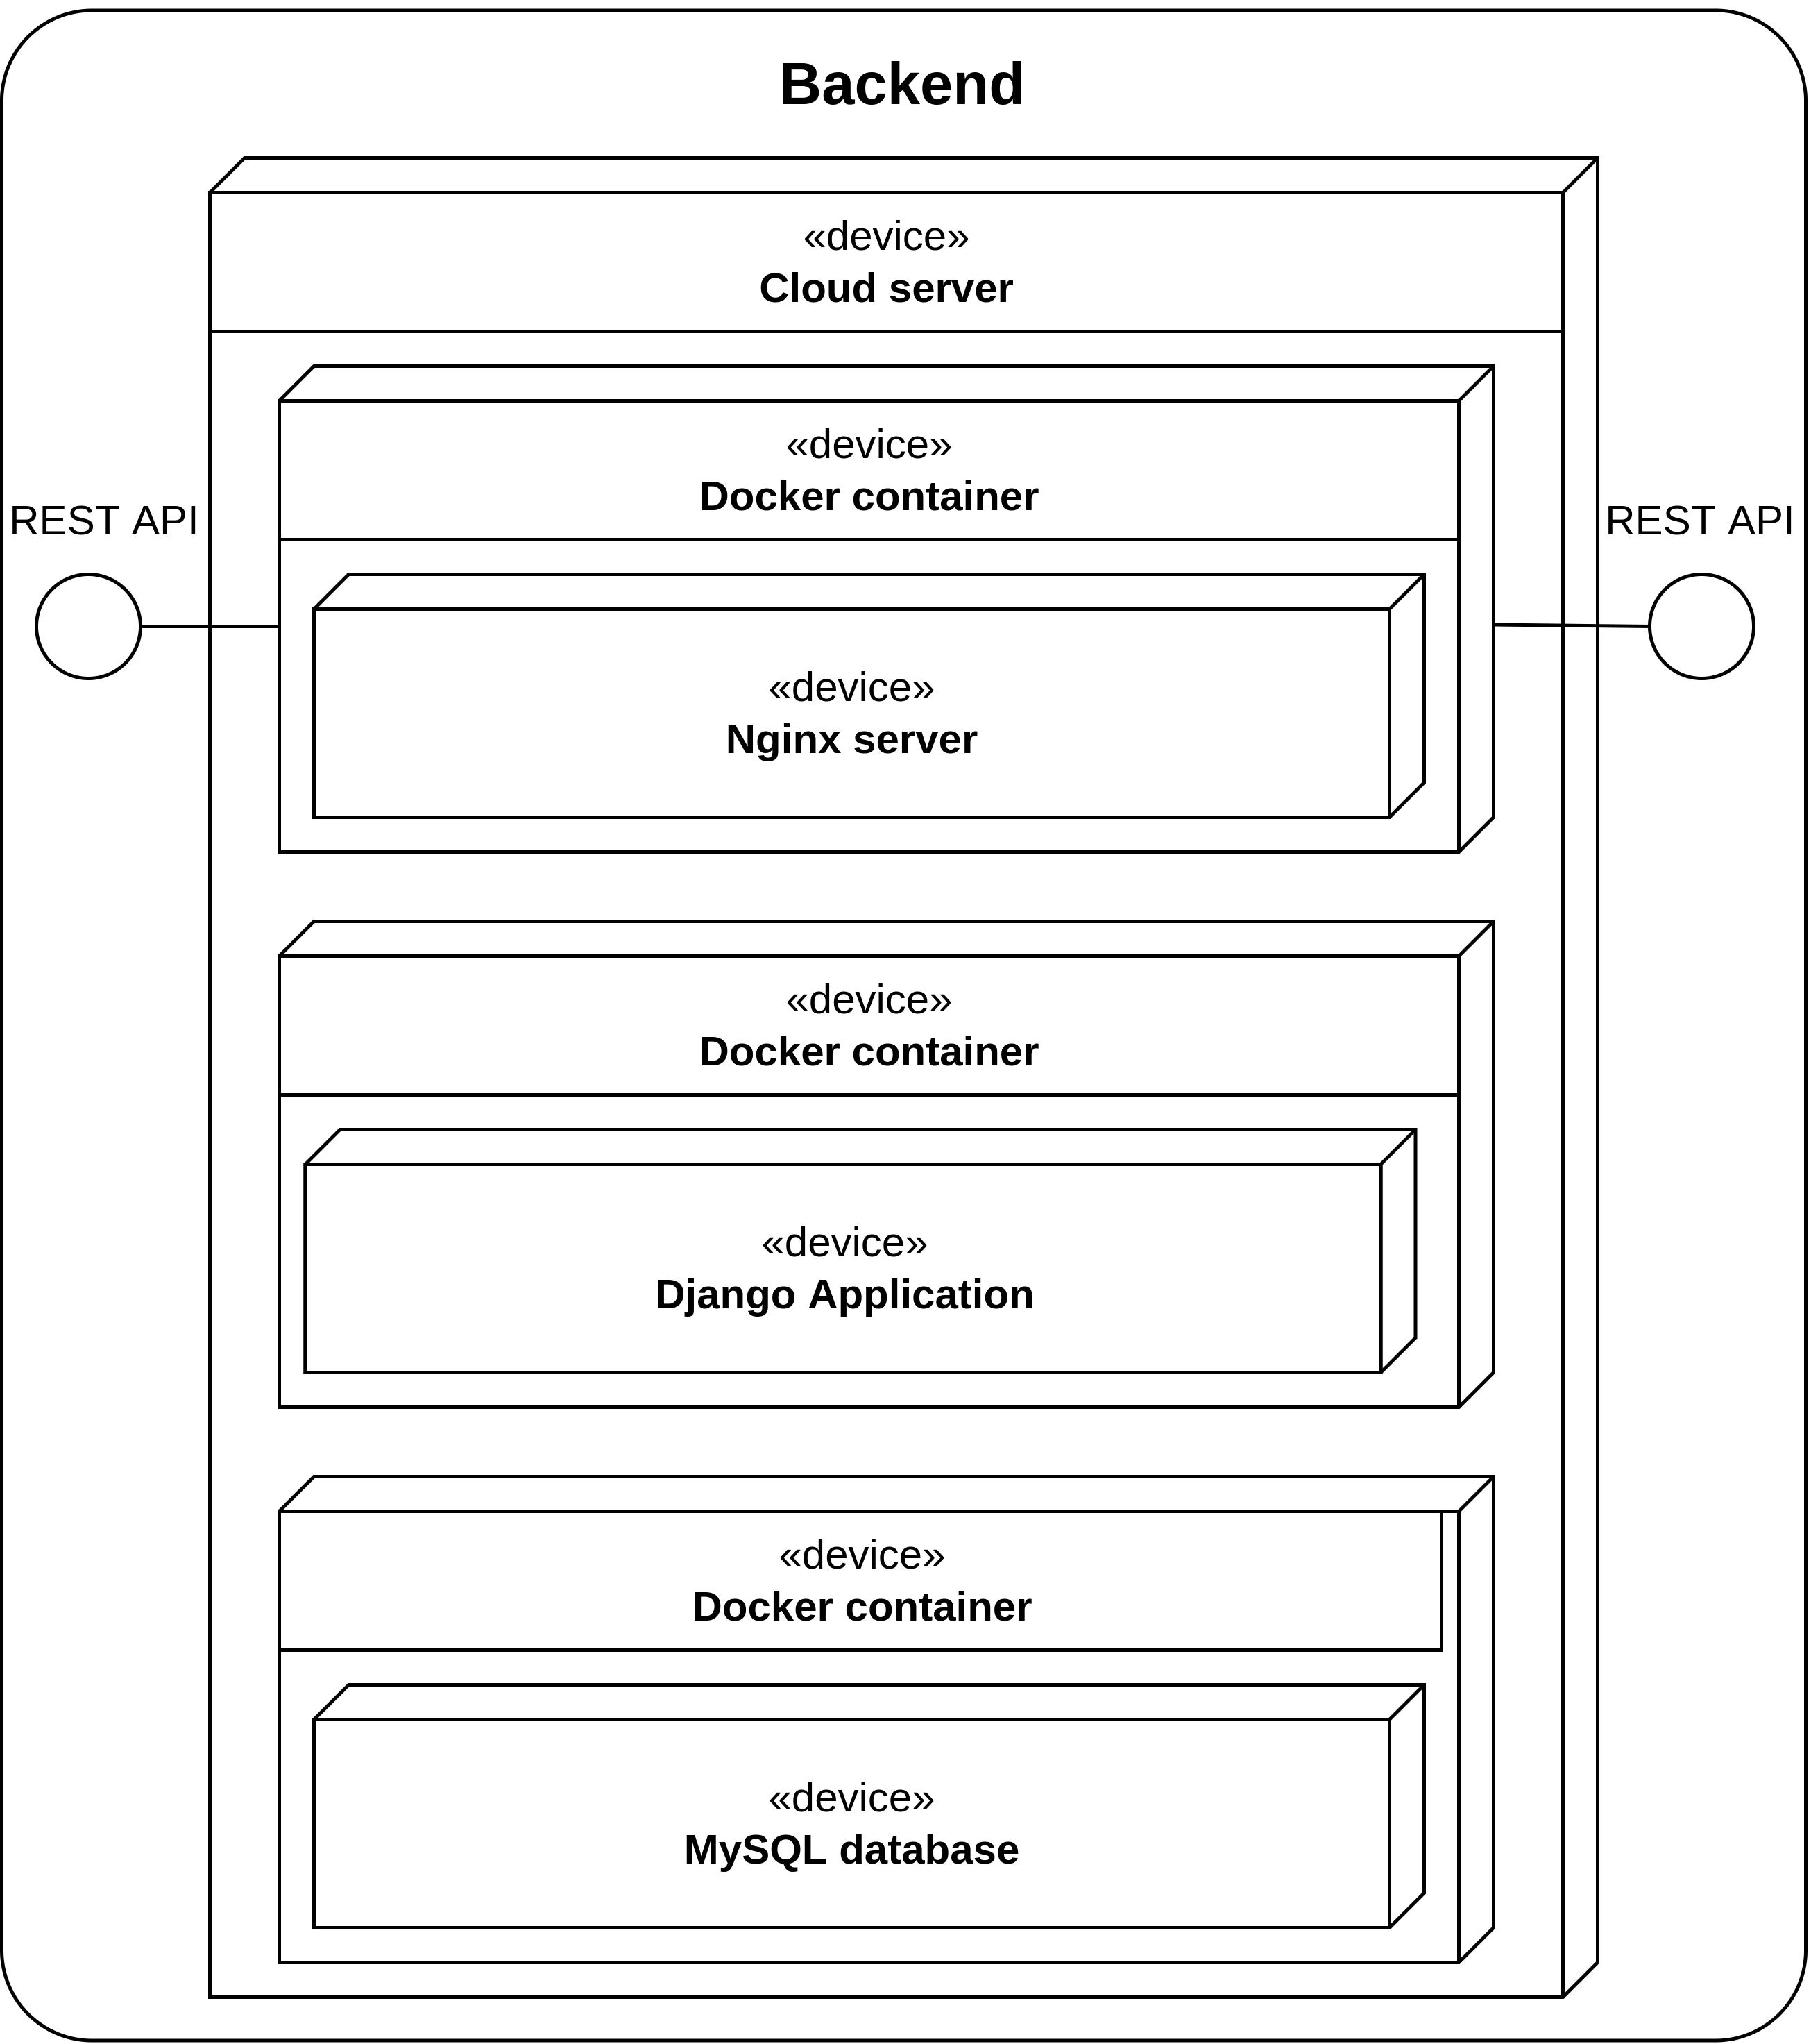
\includegraphics[width=6cm]{images/deployment_diagram_backend.drawio.png}
    \caption{Deployment diagram of the backend server software.}
    \label{fig:deployment-backend}
\end{figure}


\subsubsection{Backend application}\label{sec:backend-application}
The backend server-side application is written in the Django framework. The Django framework serves as an \ac{orm} for the database, which makes it much easier to query the database. The main purposes of the backend application is the retrieve the right information from the database and more importantly, validate if the user is authenticated and authorised to query that information. The database itself is a MySQL database.\footnote{\url{https://www.mysql.com/}} 

\paragraph{User authentication}
User authentication is an essential part of the \ac{ips} in general, due to the fact that this is the primary defence against unauthorised querying of the \ac{api}. The authentication system in the backend consists out of three \textit{views}: registering a new user (sign up), logging in a user and logging out an existing user. 

\ind If the user creates a new account with the frontend application, their record will be added to the \texttt{users}-table, but this account is not yet functional. Upon registration an email is sent to the user with an activation link. Once the user has clicked on this link, their account will be activated and can be used to log in.

\ind A user can log in via the frontend application which sends the entered \texttt{email} and \texttt{password} to the backend via an encrypted \ac{ssl}/\ac{tls}-connection. The backend validates the credentials and if they are correct, an \textit{authentication token} is generated and sent back to the frontend. This token has to be used in \textit{all} \ac{api}-requests which query or post data from and to the database. Furthermore, this token indicates if a user is logged in or not. If a token is present in the \verb|knox_authtoken|-table, a user is considered logged in. To prevent attackers to log in with this token from a separate device, the number of tokens is limited to one token per user. If someone tries to log in with the credentials of an already logged in user, an error is returned. This token also makes it possible for the frontend to implement an automatic login system for the users.

\ind From the frontend application, users are able to log themselves out. From a backend's perspective, this means deleting the authentication token from the database. In order for the logout the succeed, the authentication token has to be sent with the request. This prevents unauthorised logging out of users. 

\paragraph{Serialization of database models}
All data is transmitted in \ac{json}-format over the \ac{api}, but it cannot be directly inserted in this format in the database. One of the tasks of the backend application is \textit{serializing} the data between the \ac{json}- and database formats. This not only happens when data is queried from the database, but also when data is posted to the \ac{api}. In this direction, the serializing function becomes more important, because it \textit{validates} the sent data. The data has to match the requirements of the schema of the database (e.g. certain columns of the database are non-null, others have to be unique, etc.). If not, an error message is returned to the sender and the record will not be stored. This procedure is also the main defence against \ac{sql}-injection.

\paragraph{User roles}
All users in the database have one specific role, which is associated with a set of \textit{permissions} for this user. There are three roles: \verb|GENERATED_USER|, \verb|NORMAL_USER| and \verb|GARAGE_OWNER|. Upon registration with the frontend application, the default role is \verb|NORMAL_USER|. In order for a user to register as a \verb|GARAGE_OWNER|, the user has to provide the necessary legal documents which proves its ownership of a garage. The set of permissions of the \verb|GARAGE_OWNER| is a superset of the user permission set, with the added permissions of adding and deleting garages and adding, disabling and deleting parking lots.

\ind The \verb|GENERATED_USER| is a special role which is created upon entering of a user without an account in the parking garage. The \ac{anpr}-cameras send registered text of the licence plate to the backend. Then the backend checks if a licence plate is already registered in the database. If not, a new dummy user, with the role \verb|GENERATEED_USER| is created with the associated licence plate. This account only serves as a visualisation of the parameters of the user's park (e.g. duration) and has no functionalities which are found in a normal user's account. Upon exiting of the garage, the backend checks the associated role of the user; if it is a \verb|GENERATED_USER|, the account, with the associated licence plate, is deleted.


\clearpage

\section{Design motivation}\label{sec:design-motivation}
the design discussed in this report was not chosen without careful consideration of all options. The first decision made was which micro controller to use. Common types of micro controllers such as a Raspberry Pi or an Arduino are readily available and are suitable for the project's needs. The Raspberry Pi 3B was used because the department had it available. \\

Secondly, the detection of entering or leaving cars can be done by cameras with motion detection software. This means that the camera is constantly running and detects whether or not there is any movement. The positive side of this method is that you don't need any sensors or other extra hardware. The downside is that it might be too much to handle for the Raspberry Pi. An alternative option is working with sensors (e.g. a distance sensor) to detect the cars. This is less heavy for the Raspberry Pi, but adds an extra cost to the garage. Another option would be to leave the cameras filming and run the algorithm directly on the video footage. But this may also be too much to handle for the Raspberry Pi. Therefore, the option with the sensors is chosen for this project. \\

Thirdly, the detection of available parking spaces can be done by several sensors. The most useful ones are \ac{udms} or light sensors. The latter is more expensive and doesn't offer any extra advantages over the \ac{udms}. Therefore the \ac{udms}s (\textsc{hc-sr04}) are used in this project.\\

Fourthly, The backend application is written with Django, an open-source web framework, written in Python. The eventual decision was made based on the following concerns: 1) Python is known to all group members; 2) Django is a very explicit framework, which does not include a lot of magic features like Ruby on Rails does; 3) Django describes itself as the ``framework for perfectionists with deadlines'', which is exactly suited for the job \cite{django_website}. \\

Lastly, The frontend application will be written in Dart, with the Flutter7 framework of Google. Other valid alter-
natives were primarily JavaScript (js)-frameworks (e.g. React8 or AngularJS9). The main benefit for Flutter
over the other frameworks is that it can run on any operation system (Android, iOS, MacOS, Linux, Windows,
etc.), that it provides type safety and null safety (Dart is a strongly typed language) and that it supports
hot reloads, which makes development much easier [Flutter, 2022]. Furthermore, two of the team members
already worked with Flutter. \\

Of course the price of the different components played also a big part in the decision making. The prices of the individual components and the total price can be found in \ref{tab:budget}. The leftmost column gives the name of the component used in the
model. The second column shows how many pieces of that component are needed. Column 3 shows the price
per piece and column 4 the total price for a specific component.
The budget for this project is 250 euros. Right now the design only uses a total of 153.53 euros. You can see
this in the second to last row of Table \ref{tab:budget}. This means that the budget is not nearly reached with a surplus of
96.47 euros. \newline
\begin{table}[htp]
    \centering
    \caption{Current budget state.}
\begin{tabular}{|c|c|c|c|}
	\hline
	\textbf{Component} & \textbf{Amount} & \textbf{Price/piece} & \textbf{Total} \\
	\hline
	\textsc{dorhea} Raspberry Pi Mini Camera & 2 & 11.95 & 23.9 \\
	\hline
	Ultrasonic Module Distance & 8 & 3.95 & 31.6 \\
	\hline
	\textsc{mdf} plates 6mm & 3 & 2.4 & 7.2 \\
	\hline
	Green \textsc{led} lights & 6 & 0.35 & 2.1 \\
	\hline
	Red \textsc{led} lights & 6 & 0.33 & 1.98 \\
	\hline
	Resistors & 12 & 0.2 & 2.4 \\
	\hline
	Raspberry Pi extension cable & 2 & 4.99 & 9.98 \\
	\hline
	Micro Servo Motor & 2 & 7.21 & 14.42 \\
	\hline
    Raspberry Pi 3B & 1 & 59.95 & 59.95 \\
    \hline
	\multicolumn{2}{|c|}{Total Price} & \multicolumn{2}{c|}{153.53} \\
	\hline
	\multicolumn{2}{|c|}{Remaining} & \multicolumn{2}{c|}{96.47} \\

	\hline
\end{tabular}
        
    \label{tab:budget}
\end{table}
   \newline

\section{Case example}\label{sec:case-example}
Earlier, this report gave an abstract explanation of how the system should work and the more concrete implementation using the different components of both the software and the hard system. Subsequently, this section gives a real-world example of a user experience in the parking garage. Of course, in following reports, these actions are going to be made more concrete with sequence diagrams. Due to the large size of the flowcharts, they are included in Appendix \ref{app:flowcharts}.

The process begins with the user who drives towards the entry barrier. A \ac{udms} detects the car and sends a signal to the \textsc{anpr}-camera which takes a picture of the licence plate. This picture is then analyzed by the Google Vision \textsc{api}. The recognised string from the licence plate is then sent to the backend with a \texttt{POST}-request to \texttt{api/plate}. The system supports two use cases: either the user has a registered account with a licence plate, or the user has not. In both cases the user should be able to use the garage. The backend checks which of the two cases the received licence plate falls in. In the former, the barrier will be opened and the \verb|licence_plate|-table is updated to include the time of arrival. In the latter case, the backend will create a new user account and print a paper ticket with a \textsc{qr}-code which contains a link to the created account. With this dummy account the user can view all the information about his park. This dummy account is deleted if the users exits the garage, compliant to current \ac{gdpr}-guidelines. Figure \ref{fig:garage-enter} in Appendix \ref{app:flowcharts} shows a schematic overview of the entering process. \\

After entering the garage, the user drives to the pre-booked parking lot, in which case the occupancy of the parking lot is already set to \texttt{True} or to a parking lot of choice. In the latter case, a \ac{udms} detects the cars, so that the Raspberry Pi can sent an \ac{api}-request to backend to update the respective table. Note that only if the parking lot is booked, the parking lot is associated with the licence plate and thus with the user. Figure \ref{fig:car-detection} in Appendix \ref{app:flowcharts} shows a schematic overview of this process. \\

When exiting the garage, it is recommended that the user pays its ticket in advance, to make the exiting-process run smoothly, but the system also supports payments in front of the barrier for users who might have forgotten to pay.

\ind In a similar way as when entering, a \ac{udms} detects the car and the \ac{anpr}-camera takes a picture, which is sent to the Google Vision \ac{api} for analysis. Subsequently, the recognised text is sent to the backend via the same \textsc{url}. The backend can distinguish the images for entering and exiting the garage via the \verb|licence_plates|-tables which stores whether a licence plate is currently inside the garage. This table also contains a column which indicates if the user connected to the licence plate has already paid. If this is the case, the barrier will open. In the opposite case, there are two possibilities: the user has an account which supports automatic payments, in which case the payment will happen in situ and the barrier will open consequently. In the case in which the user hasn't paid, nor has an account which supports automatic payment, a paper ticket will be printed with a \textsc{qr}-code which redirects the user to a payment-environment. Once the user has paid its ticket, the barrier will open. Figure \ref{fig:garage-exit} in Appendix \ref{app:flowcharts} shows a schematic overview of the exiting process. \\


Note that the need of paper tickets isn't fully eliminated in this user flow, but is only used as a back-up system if the user doesn't have an account forgot to pay. In both cases, the user will be able to use our parking garage with almost the same features as a user who installed the application.

\section{System analysis}\label{sec:system analysis}

\section{Conclusion}\label{sec:coclusion}
The work of the previous weeks has led to a solid foundation on which can be built upon in the upcoming weeks. There's a concrete design of the major parts of the system, namely the frontend application, the backend server and the Raspberry Pi. Furthermore, a scale model of the parking garage has already been realised. All major functionalities of the different systems have been designed and connected to each other in theory. The main work of the forthcoming weeks is bringing the theory into practise and realising all the details of the different systems. The design will offer an answer to the problem of making a safe infrastructure that makes parking easier and faster.

\section{Course integration}\label{sec:course-integration}
% How does our project use knowledge which we've learned through our courses in the first and second year?
This project is a sequel of it's predecessors P\&O 1 and P\&O 2. So the most knowledge and experience that's been used for this project came from these courses. In these courses things like writing reports (in \LaTeX), keeping track of a logbook, making presentations, ect. were taught. These are basic aspects that are needed for creating a good project. As mentioned earlier, the experience that's been gained from these courses is also very important. From these courses the skill of working in a team were developed, which was very important for this project and will remain important for future projects. \\

\noindent Furthermore, methodology of computer science was an important course for an introduction to programming and understanding complex algorithms. This course was taught in Python and this knowledge was needed for the Raspberry Pi and licence plate recognition. Along with Python, Dart was used and this language was easy to learn because of this course.  \\

\noindent Just like methodology of computer science was used for the licence plate recognition, other courses like calculus and linear algebra were needed for neural networks. Calculus was usefull for solving the optimization problems in the neural network, to find the best solution. Linear algebra is used in the neural networks for solving large systems of linear equations. \\  

\noindent Another course that was very useful, was technical drawing for creating our physical design in Solid Edge. In this course the skills were taught for creating a 3D-design of an object or product and understanding the 2D-drawings of it. Other knowledge that was used for the physical aspect of the project was circuit design. This was taught in P\&O 2 and was used for the sensors and lights. For creating these electronic circuits, knowledge from the course electrical networks was also necessary. This course was needed for understanding how to connect different electronic components with each other.\\

\noindent Of course was the knowledge of all these courses not enough to make and realise this project. But it's a good basis to understand and learn new advanced topics in this field.  

\clearpage
\addcontentsline{toc}{section}{References}
\bibliographystyle{apalike}
\bibliography{bibliography}

\clearpage 
\begin{appendices}
\addtocontents{toc}{\protect\setcounter{tocdepth}{2}}\makeatletter
\addtocontents{toc}{%
  \begingroup
  \let\protect\l@chapter\protect\l@section
  \let\protect\l@section\protect\l@subsection
}
\makeatother


\section{General deployment diagram}\label{app:deployment-diagram}
\begin{landscape}
   \begin{figure}
    \centering
    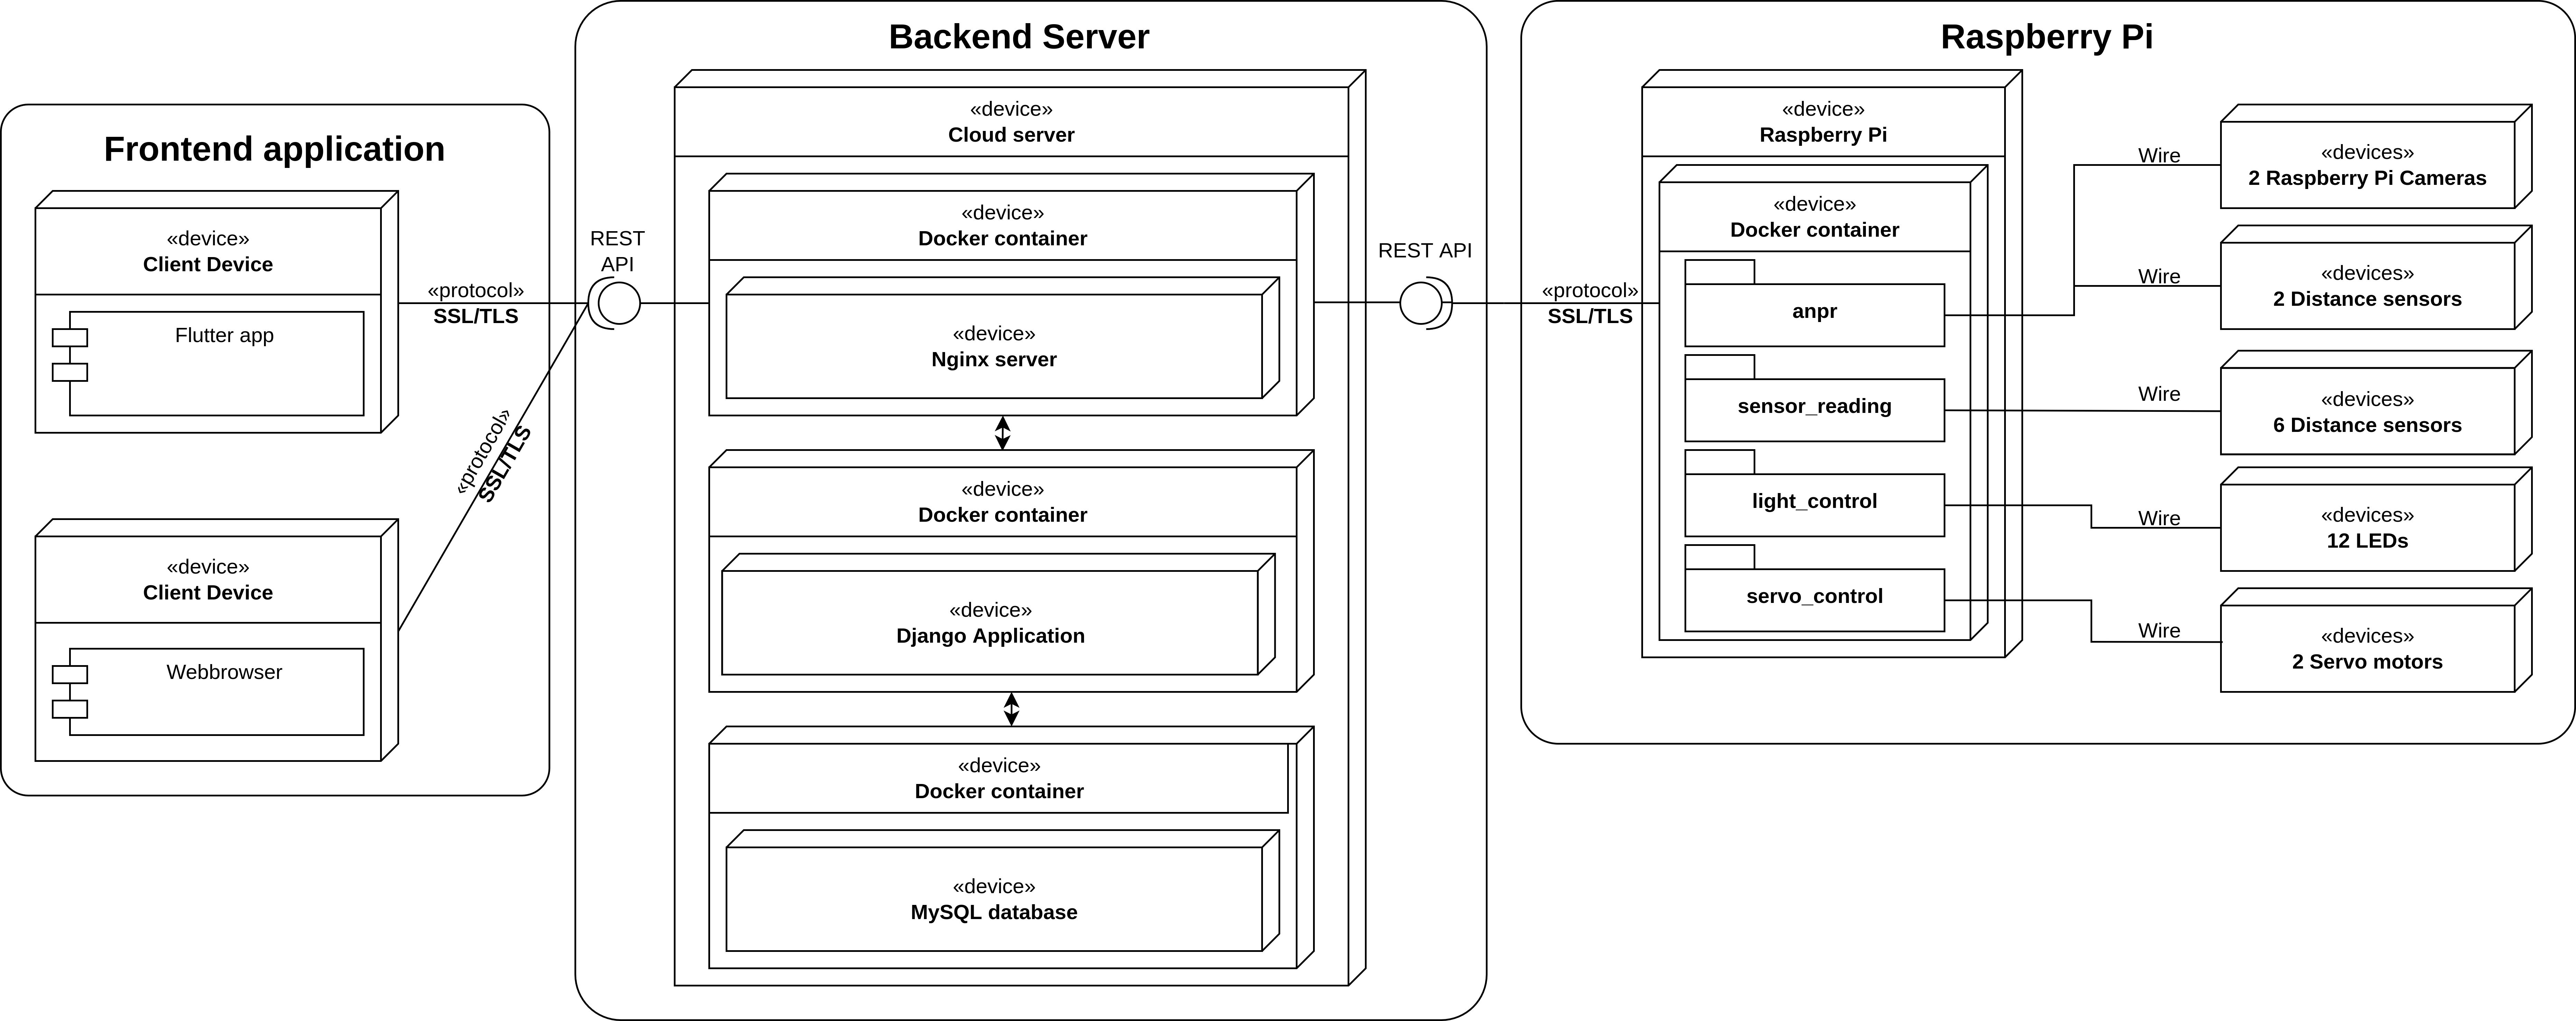
\includegraphics[width=25cm]{images/deployment_diagram.drawio.png}
    \caption{General deployment diagram.}
    \label{fig:general-deployment-diagram}
\end{figure}
\end{landscape}

\clearpage
    
\section{App diagrams}\label{app:app-diagram}
\begin{landscape}
   \begin{figure}
    \centering
    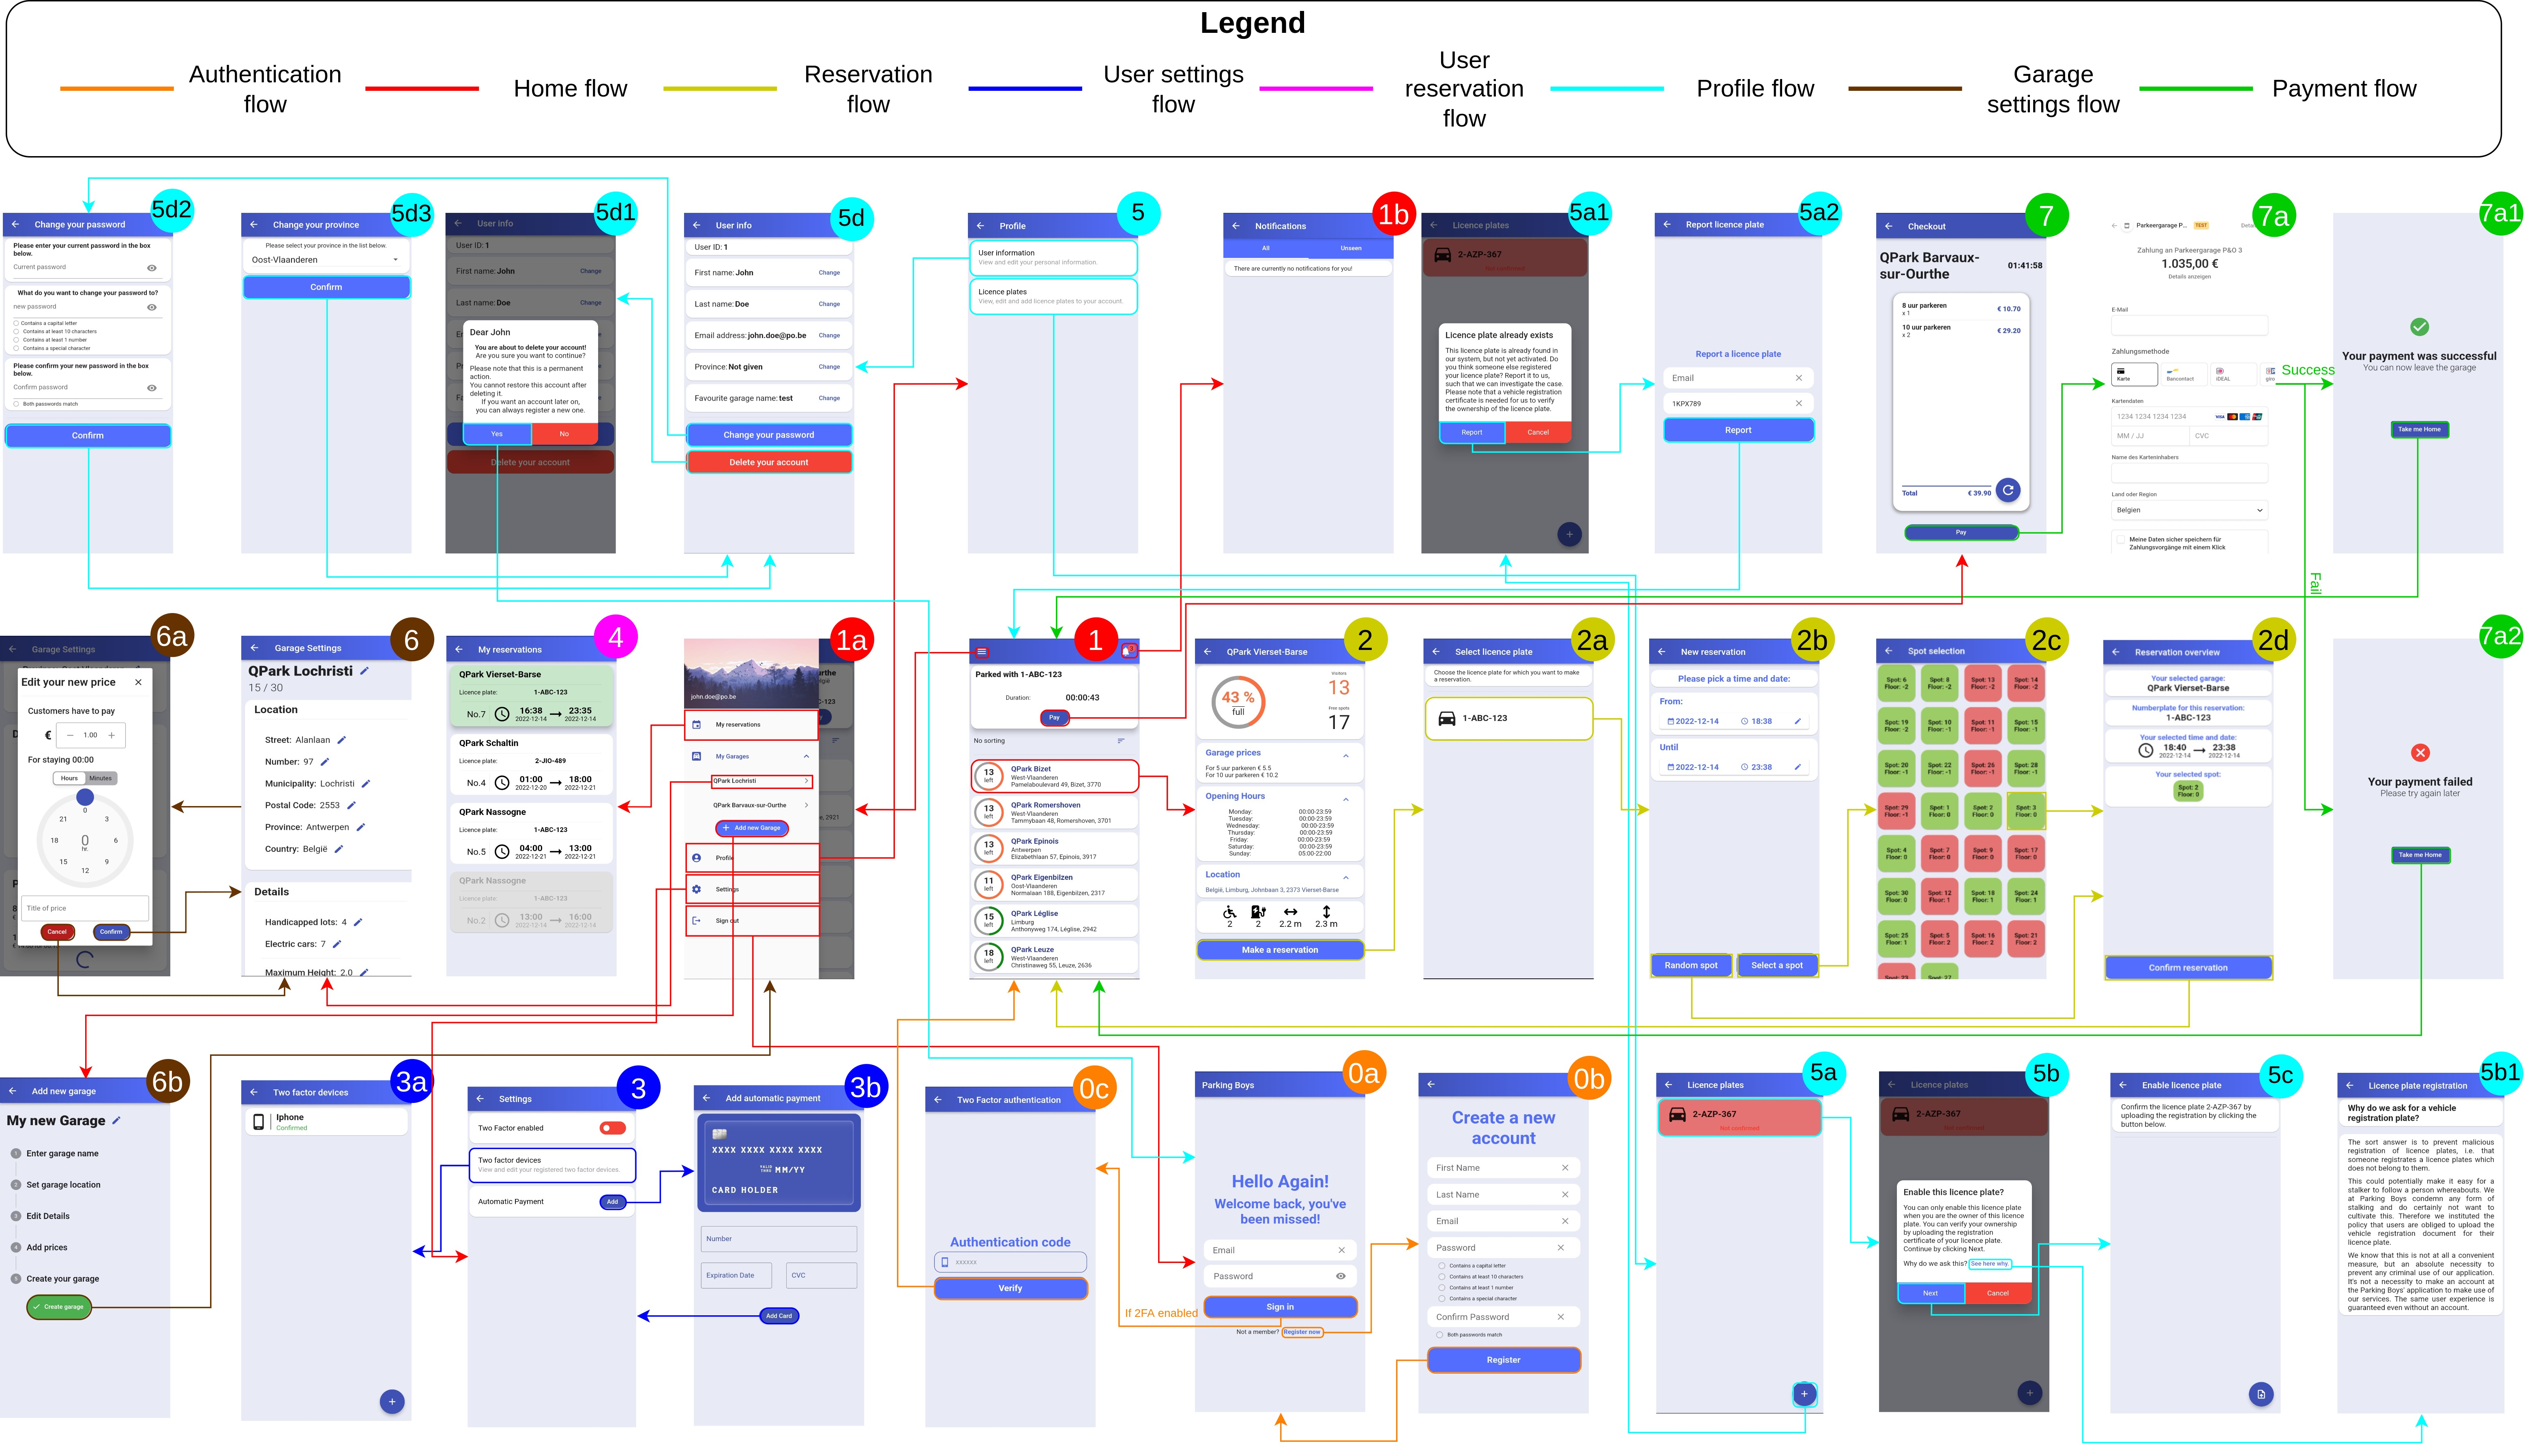
\includegraphics[width=25cm]{images/app_diagram-general.drawio}
    \caption[General app diagram.]{General app diagram which displays the user flow within the frontend application. The pages are enumerated, where a new number indicates a change of flow. Pages with the same number belong to the same logic flow within the application. The routes of the back button are not indicated with an arrow as they represent the reserve direction of the arrow which points to this page.}
    \label{fig:general-app-diagram}
\end{figure}
\end{landscape}

\clearpage
\begin{figure}[hpt]
    \centering
    \includegraphics[width=16cm]{images/app_diagram-auth-flow.drawio.png}
    \caption{App diagram of the authentication flow (Flow 0).}
    \label{fig:auth-flow}
\end{figure}
\begin{figure}[hpt]
    \centering
    \includegraphics[width=16cm]{images/app_diagram-home-flow.drawio.png}
    \caption{App diagram of the home flow (Flow 1).}
    \label{fig:home-flow}
\end{figure}

\clearpage

\begin{figure}[hpt]
    \centering
    \includegraphics[width=14cm]{images/app_diagram-reservation.drawio.png}
    \caption{App diagram of the reservation flow (Flow 2).}
    \label{fig:reservation-flow}
\end{figure}
\begin{figure}[hpt]
    \centering
    \includegraphics[width=14cm]{images/app_diagram-user-settings-flow.drawio.png}
    \caption{App diagram of the user settings flow (Flow 3).}
    \label{fig:user-settings-flow}
\end{figure}
\begin{figure}[!hpt]
    \centering
    \includegraphics[width=14cm]{images/app_diagram-user-reservation-flow.drawio.png}
    \caption{App diagram of the user reservation flow (Flow 4).}
    \label{fig:user-reservation-flow}
\end{figure}

\clearpage

\begin{figure}[hpt]
    \centering
    \includegraphics[width=16cm]{images/app_diagram-profile-flow.drawio.png}
    \caption{App diagram of the profile flow (Flow 5).}
    \label{fig:profile-flow}
\end{figure}
\begin{figure}[hpt]
   \centering
   \includegraphics[width=16cm]{images/app_diagram-garage-settings-flow.drawio.png}
    \caption{App diagram of the garage settings flow (Flow 6).}
   \label{fig:garage-settings-flow}
\end{figure}
\begin{figure}[!hpt]
    \centering
    \includegraphics[width=16cm]{images/app_diagram-payment.drawio.png}
    \caption{App diagram of the payment flow (Flow 7).}
    \label{fig:payment-flow}
\end{figure}

\clearpage

\begin{figure}[htp]
     \centering
     \begin{subfigure}[b]{0.30\textwidth}
         \centering
         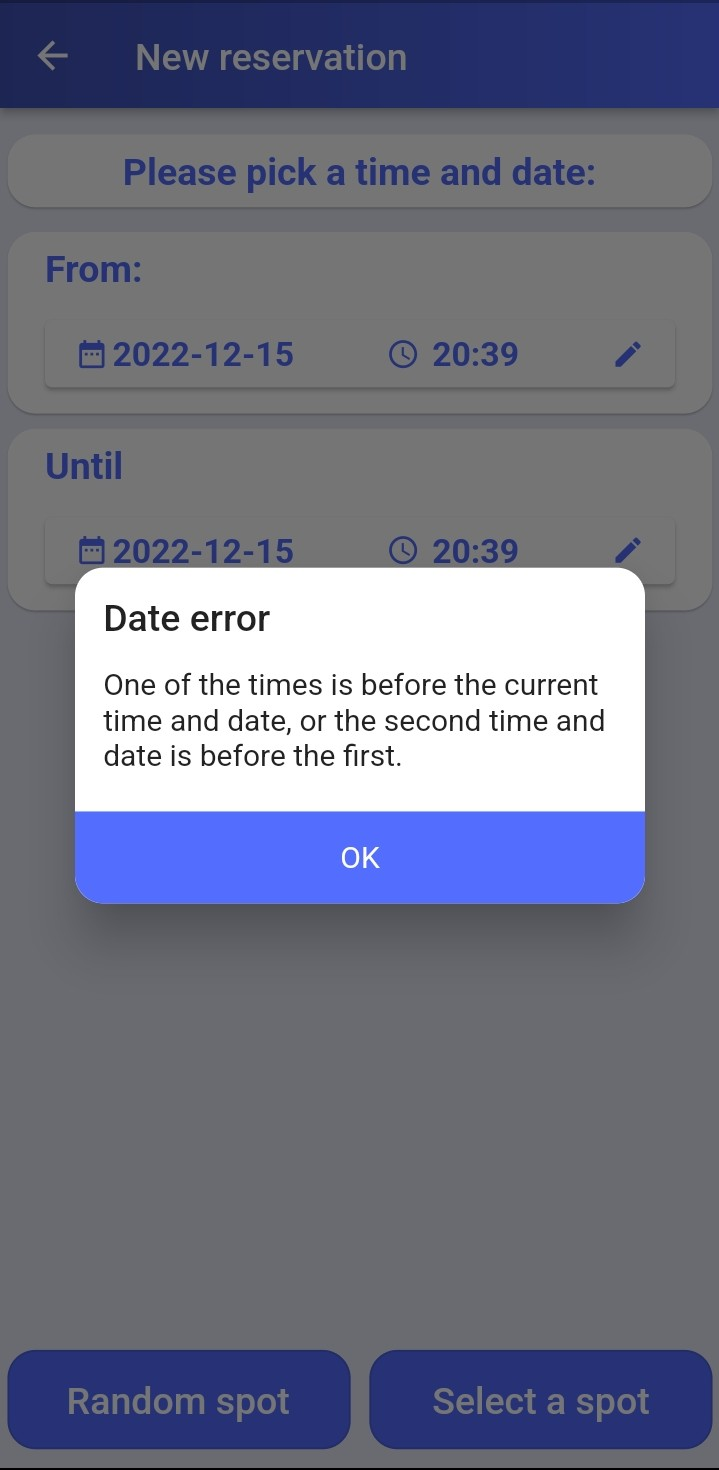
\includegraphics[width=\textwidth]{images/dialog1.jpg}
     \end{subfigure}
     \hfill
     \begin{subfigure}[b]{0.30\textwidth}
         \centering
         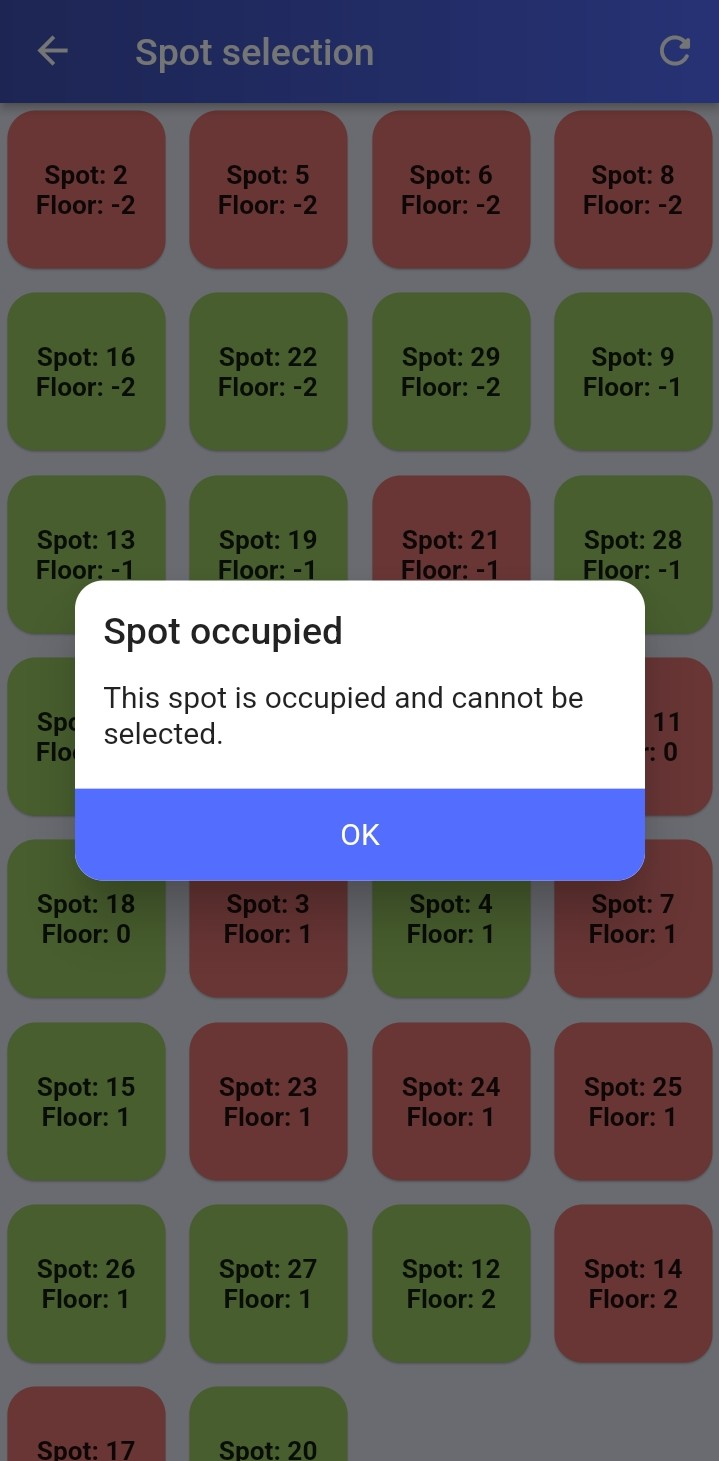
\includegraphics[width=\textwidth]{images/dialog2.jpg}
     \end{subfigure}
        \caption{Examples of error pop ups in the frontend application.}
        \label{fig:error-dialogs}
\end{figure}
\begin{figure}[!htp]
     \centering
     \begin{subfigure}[b]{0.30\textwidth}
         \centering
         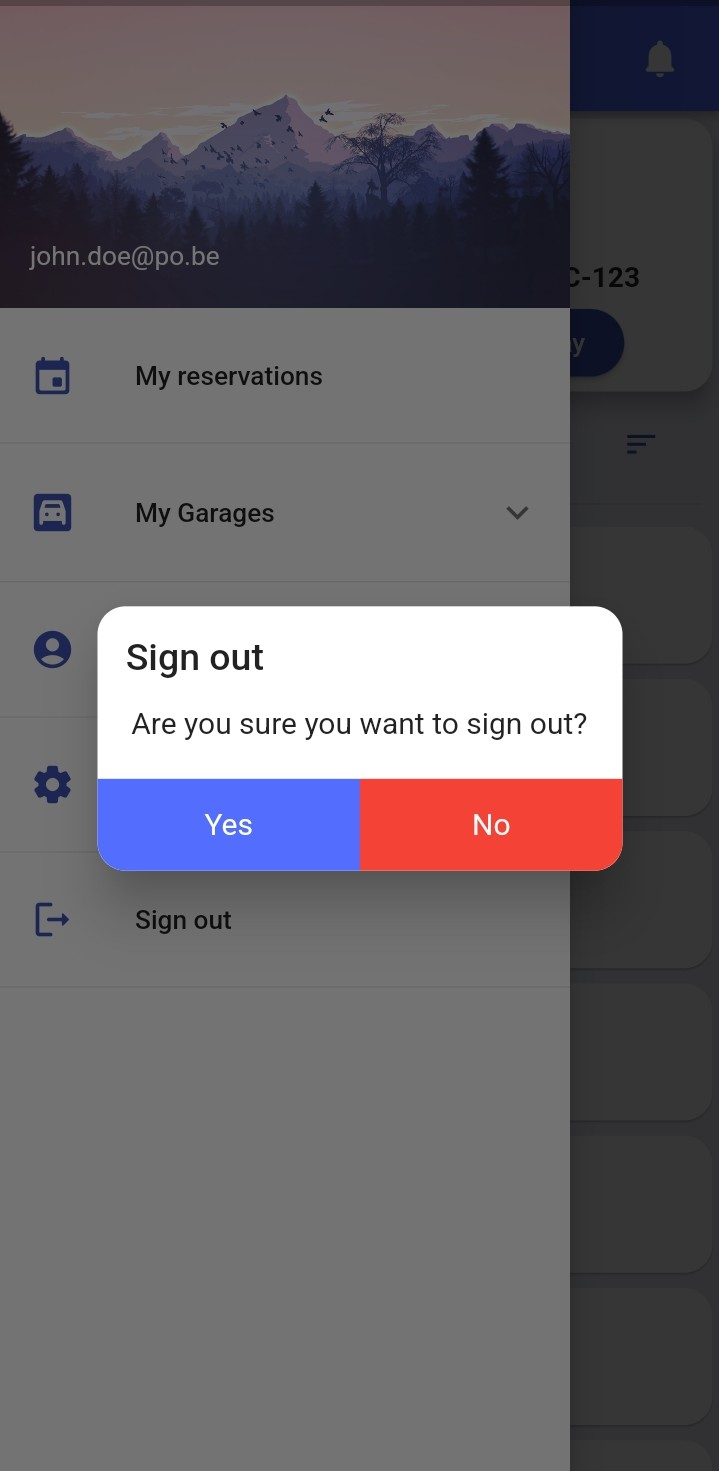
\includegraphics[width=\textwidth]{images/dialog3.jpg}
     \end{subfigure}
     \hfill
     \begin{subfigure}[b]{0.30\textwidth}
         \centering
         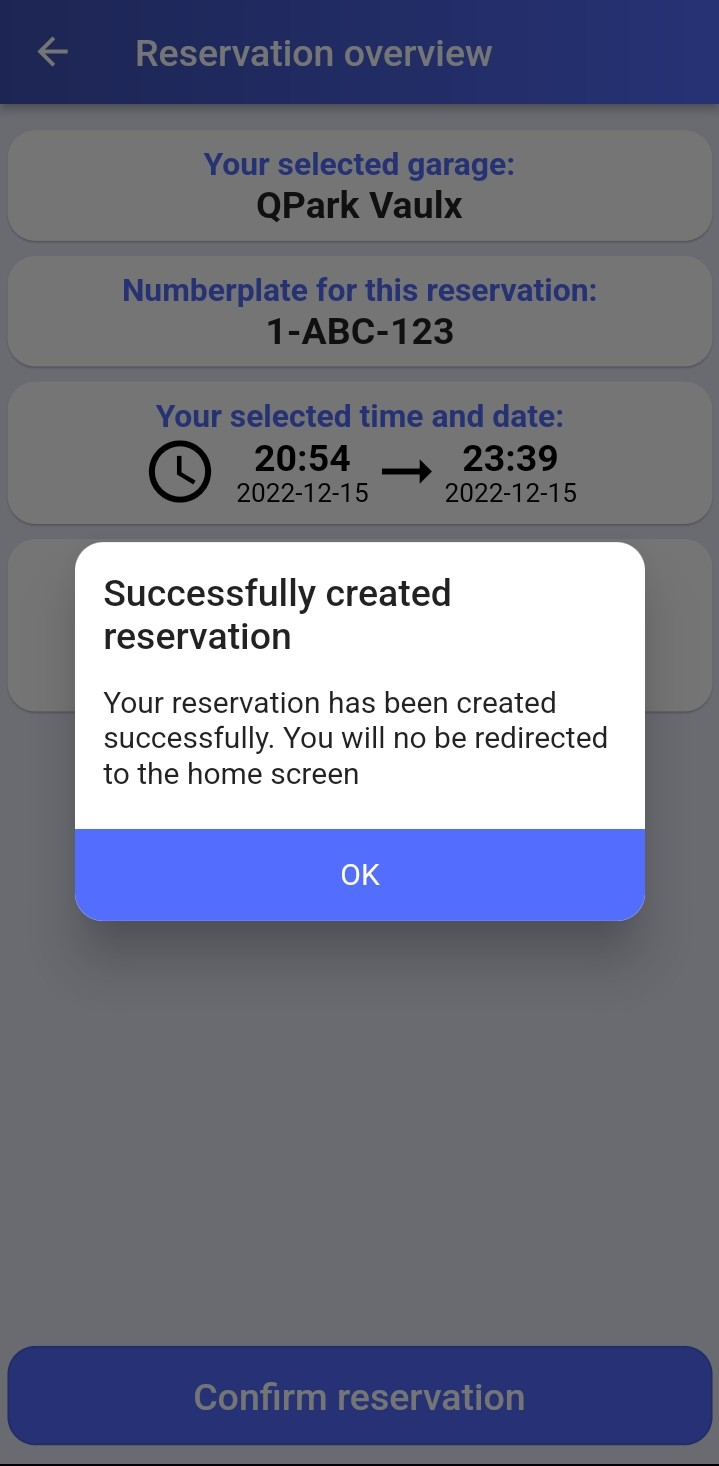
\includegraphics[width=\textwidth]{images/dialog4.jpg}
     \end{subfigure}
        \caption{Examples of information pop ups in the frontend application.}
        \label{fig:information-dialogs}
\end{figure}

\clearpage

\begin{table}[hpt]
    \centering
    \begin{tabular}{|c|c|p{9cm}|}
    \hline
         \textbf{Page code}& \textbf{Page name} & \textbf{Short description} \\
         \hline
         \hline
         0a & Login page & Lets the user enter their email and password and authenticates it with the backend.\\
         \hline 
         0b & Register page & Allows the creation of new accounts by inputting all necessary information by the user.\\
         \hline 
         0c & \ac{2fa} Page & Allows the user to enter the \ac{2fa}-code from their \ac{totp}-device. \\
         \hline 
         \hline
         1 & Home page & Central page in the application which is the entry point for all major flows.\\
         \hline 
         1a & Home banner & Banner which allows the user to navigate to all important flows and to sign out. \\
         \hline 
         \hline
         2 & Garage info page & Provides an overview of all information about a garage, including its occupancy, prices and opening hours. Is the entry point for the reservation flow.\\
         \hline 
         2a & Licence plate selection page & Allows the user to select for which licence plate they want to make a reservation. \\
         \hline 
         2b & Make reservation page & Allows the user to enter their start and end time of the reservation they want to make. Validates them before continuing. \\
         \hline 
         2c & Spot selection page & Allows the user to choose a parking lot for which they want to make a reservation. \\
         \hline 
         2d & Reservation overview page &  Provides an overview of the reservation the user is about to make. On confirm, the user is redirected to the home page \\
         \hline 
         \hline
         3 & Settings page & Entry point for the users altering the user settings. \\
         \hline 
         3a & Two factor devices page & Allows the user to add, update or delete \ac{totp}-devices. \\
         \hline 
         3b & Add automatic payment page& Allows the user to enter their credit card details, which enables automatic payment.\\
         \hline 
         \hline
         4 & User reservation page & Overview of the user's reservations, highlighting the current reservation and disabling past reservations.\\
         \hline 
         \hline
         5 & Profile page & Entry point for altering and viewing user information. \\
         \hline 
         5a & Licence plates page & Allows the user to view, add and confirm licence plates. \\
         \hline 
         5b & Confirm licence plate dialog& Allows the user to choose to enable their licence plate. \\
         \hline 
         5b1 & Registration explication page & Explains the user why a vehicle registration document is necessary for the application to enable their licence plate.\\
         \hline 
         5c & Confirm licence plate page & Allows the user to upload a vehicle registration document to enable their licence plate.\\
         \hline 
         5d & User info page & Allows the user to view and edit their personal information. \\
         \hline 
         5d1 & User deletion pop up & Allows the user to choose if they want to delete their account. \\
         \hline 
         5d2 & Change password page & Allows the user to change their password by entering a new one. \\
         \hline 
         5d3 & Change province page & Allows the user to change their location.\\
         \hline 
         \hline
         6 & Garage settings page & Allows a garage owner to alter the information about their garage, including the parking lots, prices, opening hours and location. \\
         \hline 
         6a & Add prices page & Allows a garage owner to add new prices to their garage. The prices will be synchronised with the Stripe servers.\\
         \hline 
         \hline
         7 & Checkout page & Provides an overview of the due amount and the parked time to the user.\\
         \hline 
         7a & Payment page & Allows the user to pay their parking bill \\
         \hline 
         7a1 & Payment success page & Provides confirmation to the user that their payment was successful. \\
         \hline 
         7a2 & Payment failed page page & Provides confirmation to the user that their payment as unsuccessful. \\
         \hline 
    \end{tabular}
    \caption[An overview of all the different pages in the frontend application.]{An overview of all the different pages in the frontend application, together with their page code and a short description.}
    \label{tab:app-pages}
\end{table}

\clearpage

\section{Mechanical part list}\label{app:part-list}

\begin{table}[htp]
    \centering
    \caption{Overview of all used mechanical components and their model number.}
    \begin{tabular}{|c|c|c|}
        \hline
         \textbf{Component name} & \textbf{Model number} & \textbf{Amount}  \\
         \hline
         \hline
         Raspberry Pi & Model 3B & 2 \\
         \hline
         \textsc{dorhea} Raspberry Pi Mini Kamera & \textsc{he0304-002} & 2 \\
         \hline
         Ultrasonic distance measuring sensor & \textsc{hc-sr04} & 8 \\
         \hline
         \textsc{Micro servo motor} & \textsc{oky8003} & 2 \\
         \hline
         Red \textsc{led} ($3 \ \text{mm}$) & \textsc{com-00533} & 6 \\
         \hline
         Green \textsc{led} ($3 \ \text{mm}$) & \textsc{com-09560} & 6 \\
         \hline
         Resistors ($20 \ \text{k}\Omega$) & \textsc{sfr2500002002fr500} & 12 \\
         \hline
         Jumper cables & / & $\approx 40$ \\
         \hline
         Raspberry Pi camera extension cable & \textsc{b087dfJ2rp} & 2 \\
         \hline
         LCD screen & ST7735 & 1
         \\
         \hline
         \end{tabular}
    \label{tab:part_list}
\end{table}
\clearpage

\section{Backend API slugs}\label{app:backend-api-slugs}
\begin{table}[htp]
    \centering
    \begin{tabular}{|l|l|p{7cm}|}
        \hline
         \textbf{Slug} & \textbf{Methods} & \textbf{Short Description}  \\
         \hline
         \hline
         \texttt{api/user} &  \texttt{GET}, \texttt{PUT}, \texttt{DELETE} & Get, update or delete user information.\\
        \hline
        \texttt{api/user/change-password} &  \texttt{PUT} & Update a user's password, provided the old one.\\
        \hline
        \texttt{api/garages} &  \texttt{GET}, \texttt{POST}& Get all the available garages or post a new one.\\
        \hline
        \texttt{api/garage/<int:pk>} &  \texttt{GET}, \texttt{PUT}, \texttt{DELETE
        } & Get, update or delete information about a single garage.\\
        \hline
        \texttt{api/prices/<int:pk>} &  \texttt{GET}, \texttt{PUT}, \texttt{DELETE
        } & Get all the prices for a garage with id \texttt{pk}.\\
        \hline
        \texttt{api/opening-hours/<int:pk>} &  \texttt{GET}, \texttt{POST} & Get all the opening hours for a garage with id \texttt{pk} or add a new one.\\
        \hline
        \texttt{api/opening-hour/<int:pk>} &  \texttt{PUT}, \texttt{DELETE} & Update or delete opening hours with id \texttt{pk}.\\
        \hline
        \texttt{api/parking-lots/<int:pk>} &  \texttt{GET} & Get all the parking lots for a garage with id \texttt{pk}.\\
        \hline
        \texttt{api/parking-lot/<int:pk>} &  \texttt{GET}, \texttt{PUT}, \texttt{DELETE
        } & Get update or delete a parking lot with id \texttt{pk}. \\
        \hline
        \texttt{api/assign-parking-lot/<int:pk>} &  \texttt{GET} & Get a random free parking lot in the garage with id \texttt{pk}, given a start and end date. \\
        \hline
        \texttt{api/garage-settings/<int:pk>} &  \texttt{GET}, \texttt{PUT}, \texttt{DELETE
        } & Get, update or delete the garage settings of a garage with id \texttt{pk}.\\
        \hline
        \texttt{api/licence-plates} &  \texttt{GET}, \texttt{POST} & Get all licence plates for a user or add a new one.\\
        \hline
        \texttt{api/licence-plate/<int:pk>} &  \texttt{GET}, \texttt{PUT}, \texttt{DELETE} & Get, update or delete a licence plate with id \texttt{pk}. \\
        \hline
        \texttt{api/reservations} &  \texttt{GET}, \texttt{POST} & Get all user's reservations or add a new one.\\
        \hline
        \texttt{api/reservation/<int:pk>} &  \texttt{PUT}, \texttt{DELETE
        } & Update or delete a notification with id \texttt{pk}.\\
        \hline
        \texttt{api/notifications/<int:pk>} &  \texttt{GET} & Get all user's notifications.\\
        \hline
        \texttt{api/notification/<int:pk>} &  \texttt{PUT}, \texttt{DELETE
        } & Update or delete a notification with id \texttt{pk}.\\
        \hline
        \end{tabular}
    \caption{Overview of all general \ac{url} slugs which are supported by the backend application.}
    \label{tab:my_label}
\end{table}


\begin{table}[htp]
    \centering
    \begin{tabular}{|l|l|p{7cm}|}
    \hline
    \textbf{Slug} & \textbf{Methods} & \textbf{Short Description}  \\
    \hline
    \hline
        \texttt{api/auth/login} &  \texttt{POST} & Login a user given a email and password.\\
        \hline
        \texttt{api/auth/logout} &  \texttt{POST} & Logout a user, deleting its auth token.\\
        \hline
        \texttt{api/auth/activate-account} &  \texttt{GET} & Activate a user's account.\\
        \hline
        \texttt{api/auth/totp/disable} &  \texttt{POST} & Disable \ac{2fa} for a user.\\
        \hline
        \texttt{api/auth/totp} &  \texttt{GET}, \texttt{POST} & Get all the user's \ac{totp}-devices or add a new one.\\
        \hline
        \texttt{api/auth/totp/<int:pk>} &  \texttt{PUT}, \texttt{DELETE} & Update or delete a \ac{totp}-device with id \texttt{pk}.\\
        \hline
        \texttt{api/auth/totp/login/<int:code>} & \texttt{POST} & Post the \ac{2fa}-code to verify the user (\texttt{code} is a six-digit number).\\
        \hline
    \end{tabular}
    \caption{Overview of all \ac{url} slugs for authentication which are supported by the backend application.}
    \label{tab:my_label}
\end{table}


\begin{table}[htp]
    \centering
    \begin{tabular}{|l|l|p{7cm}|}
        \hline
    \textbf{Slug} & \textbf{Methods} & \textbf{Short Description}  \\
    \hline
        \hline
        \texttt{api/rpi/images} &  \texttt{POST} & Post the image taken by the Raspberry Pi to the backend for image analysis.\\
        \hline
        \texttt{api/rpi/parking-lot} &  \texttt{GET} & Get the parking lots from the garage where the Raspberry Pi is installed.\\
        \hline
            \end{tabular}
    \caption{Overview of all \ac{url} slugs for the local garage system, which are supported by the backend application.}
    \label{tab:url-rpi}
\end{table}


\begin{table}[htp]
    \centering
    \begin{tabular}{|l|l|p{7cm}|}
        \hline
    \textbf{Slug} & \textbf{Methods} & \textbf{Short Description}  \\
    \hline
        \hline
        \texttt{api/checkout/create-session} &  \texttt{POST} & Create a checkout session for the user to pay.\\
        \hline
        \texttt{api/checkout/preview} &  \texttt{GET} & Get the items which the user has to pay (i.e. time quantities parked).\\
        \hline
        \texttt{api/checkout/webhook} &  \texttt{POST} & Listen to incoming requests from the Stripe servers for checkout updates.\\
        \hline
        \texttt{api/stripe-connection} &  \texttt{POST} & Add or remove customers from Stripe.\\
        \hline
        \texttt{api/invoice/webhook} &  \texttt{POST} & Post the image taken by the Raspberry Pi to the backend for image analysis.\\
        \hline
        \texttt{api/rpi/parking-lot} &  \texttt{GET} & Listen to invoice updates from the Stripe servers.\\
        \hline
    \end{tabular}
    \caption{Overview of all \ac{url} slugs for payment which are supported by the backend application.}
    \label{tab:url-payment}
\end{table}

\section{Flowcharts}\label{app:flowcharts}

\begin{figure}[htp]
    \centering
    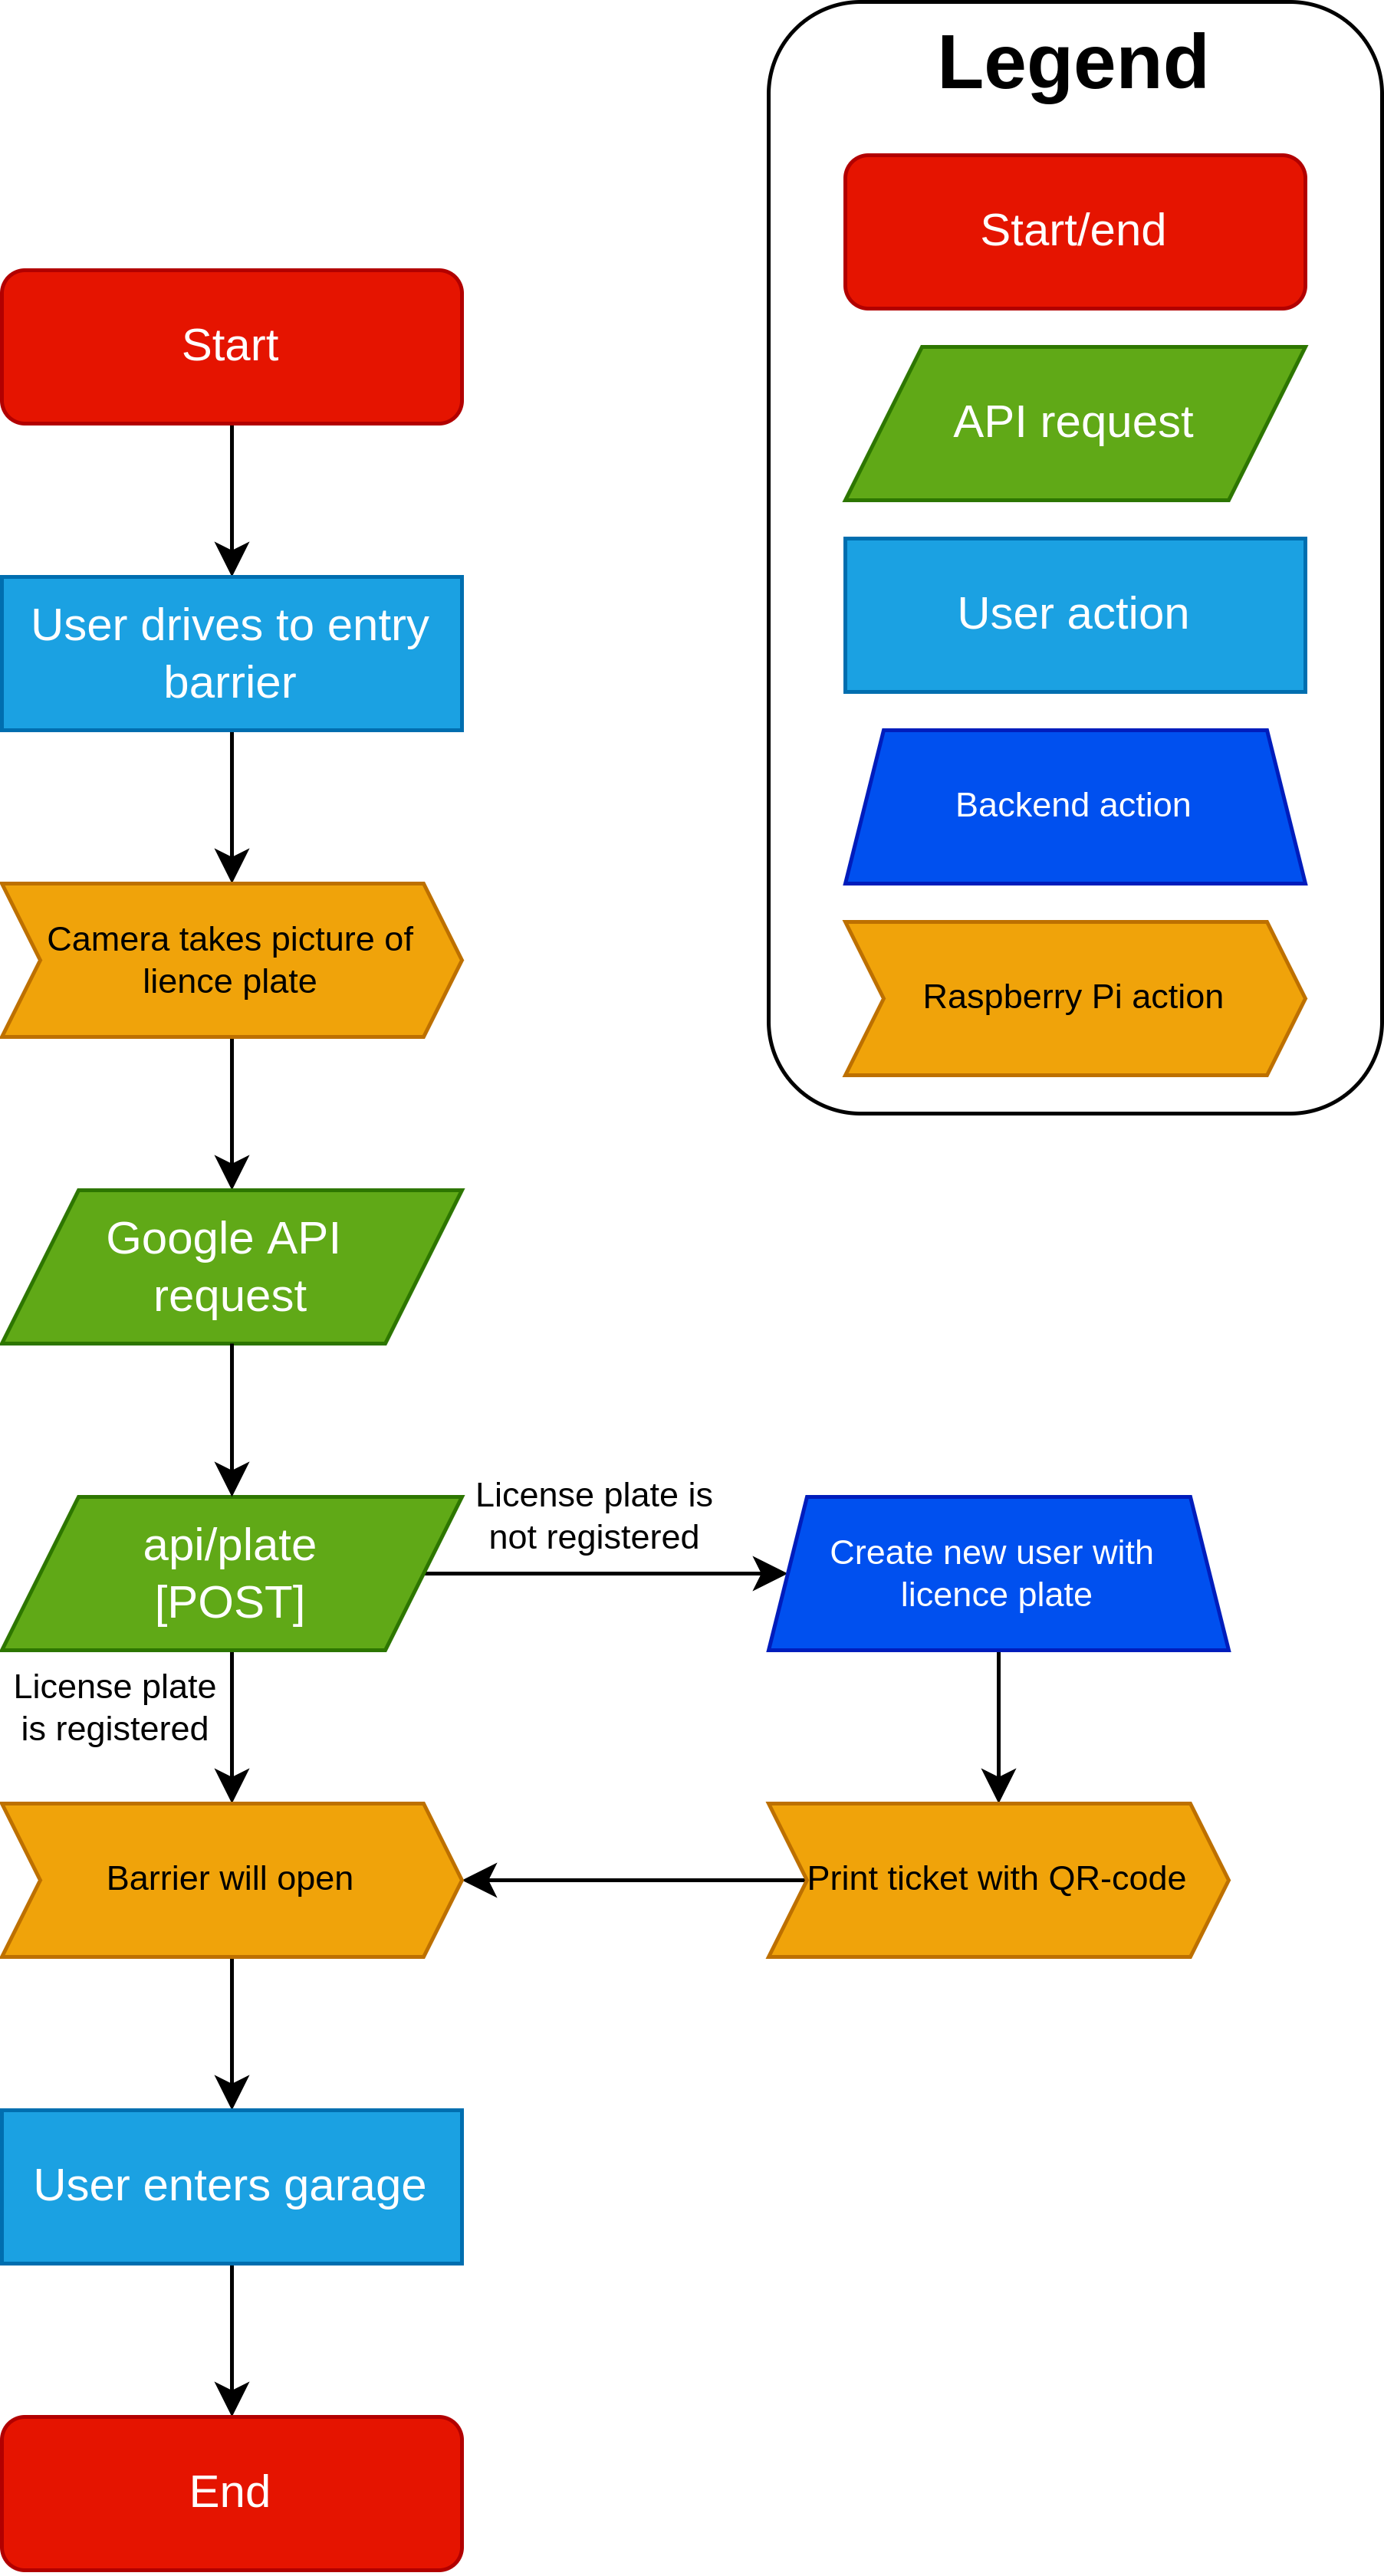
\includegraphics[width=7cm]{images/garage_enter.drawio.png}
    \caption{Flowchart of the entering process of the garage in both hardware, software and user terms.}
    \label{fig:garage-enter}
\end{figure}

\begin{figure}[htp]
    \centering
    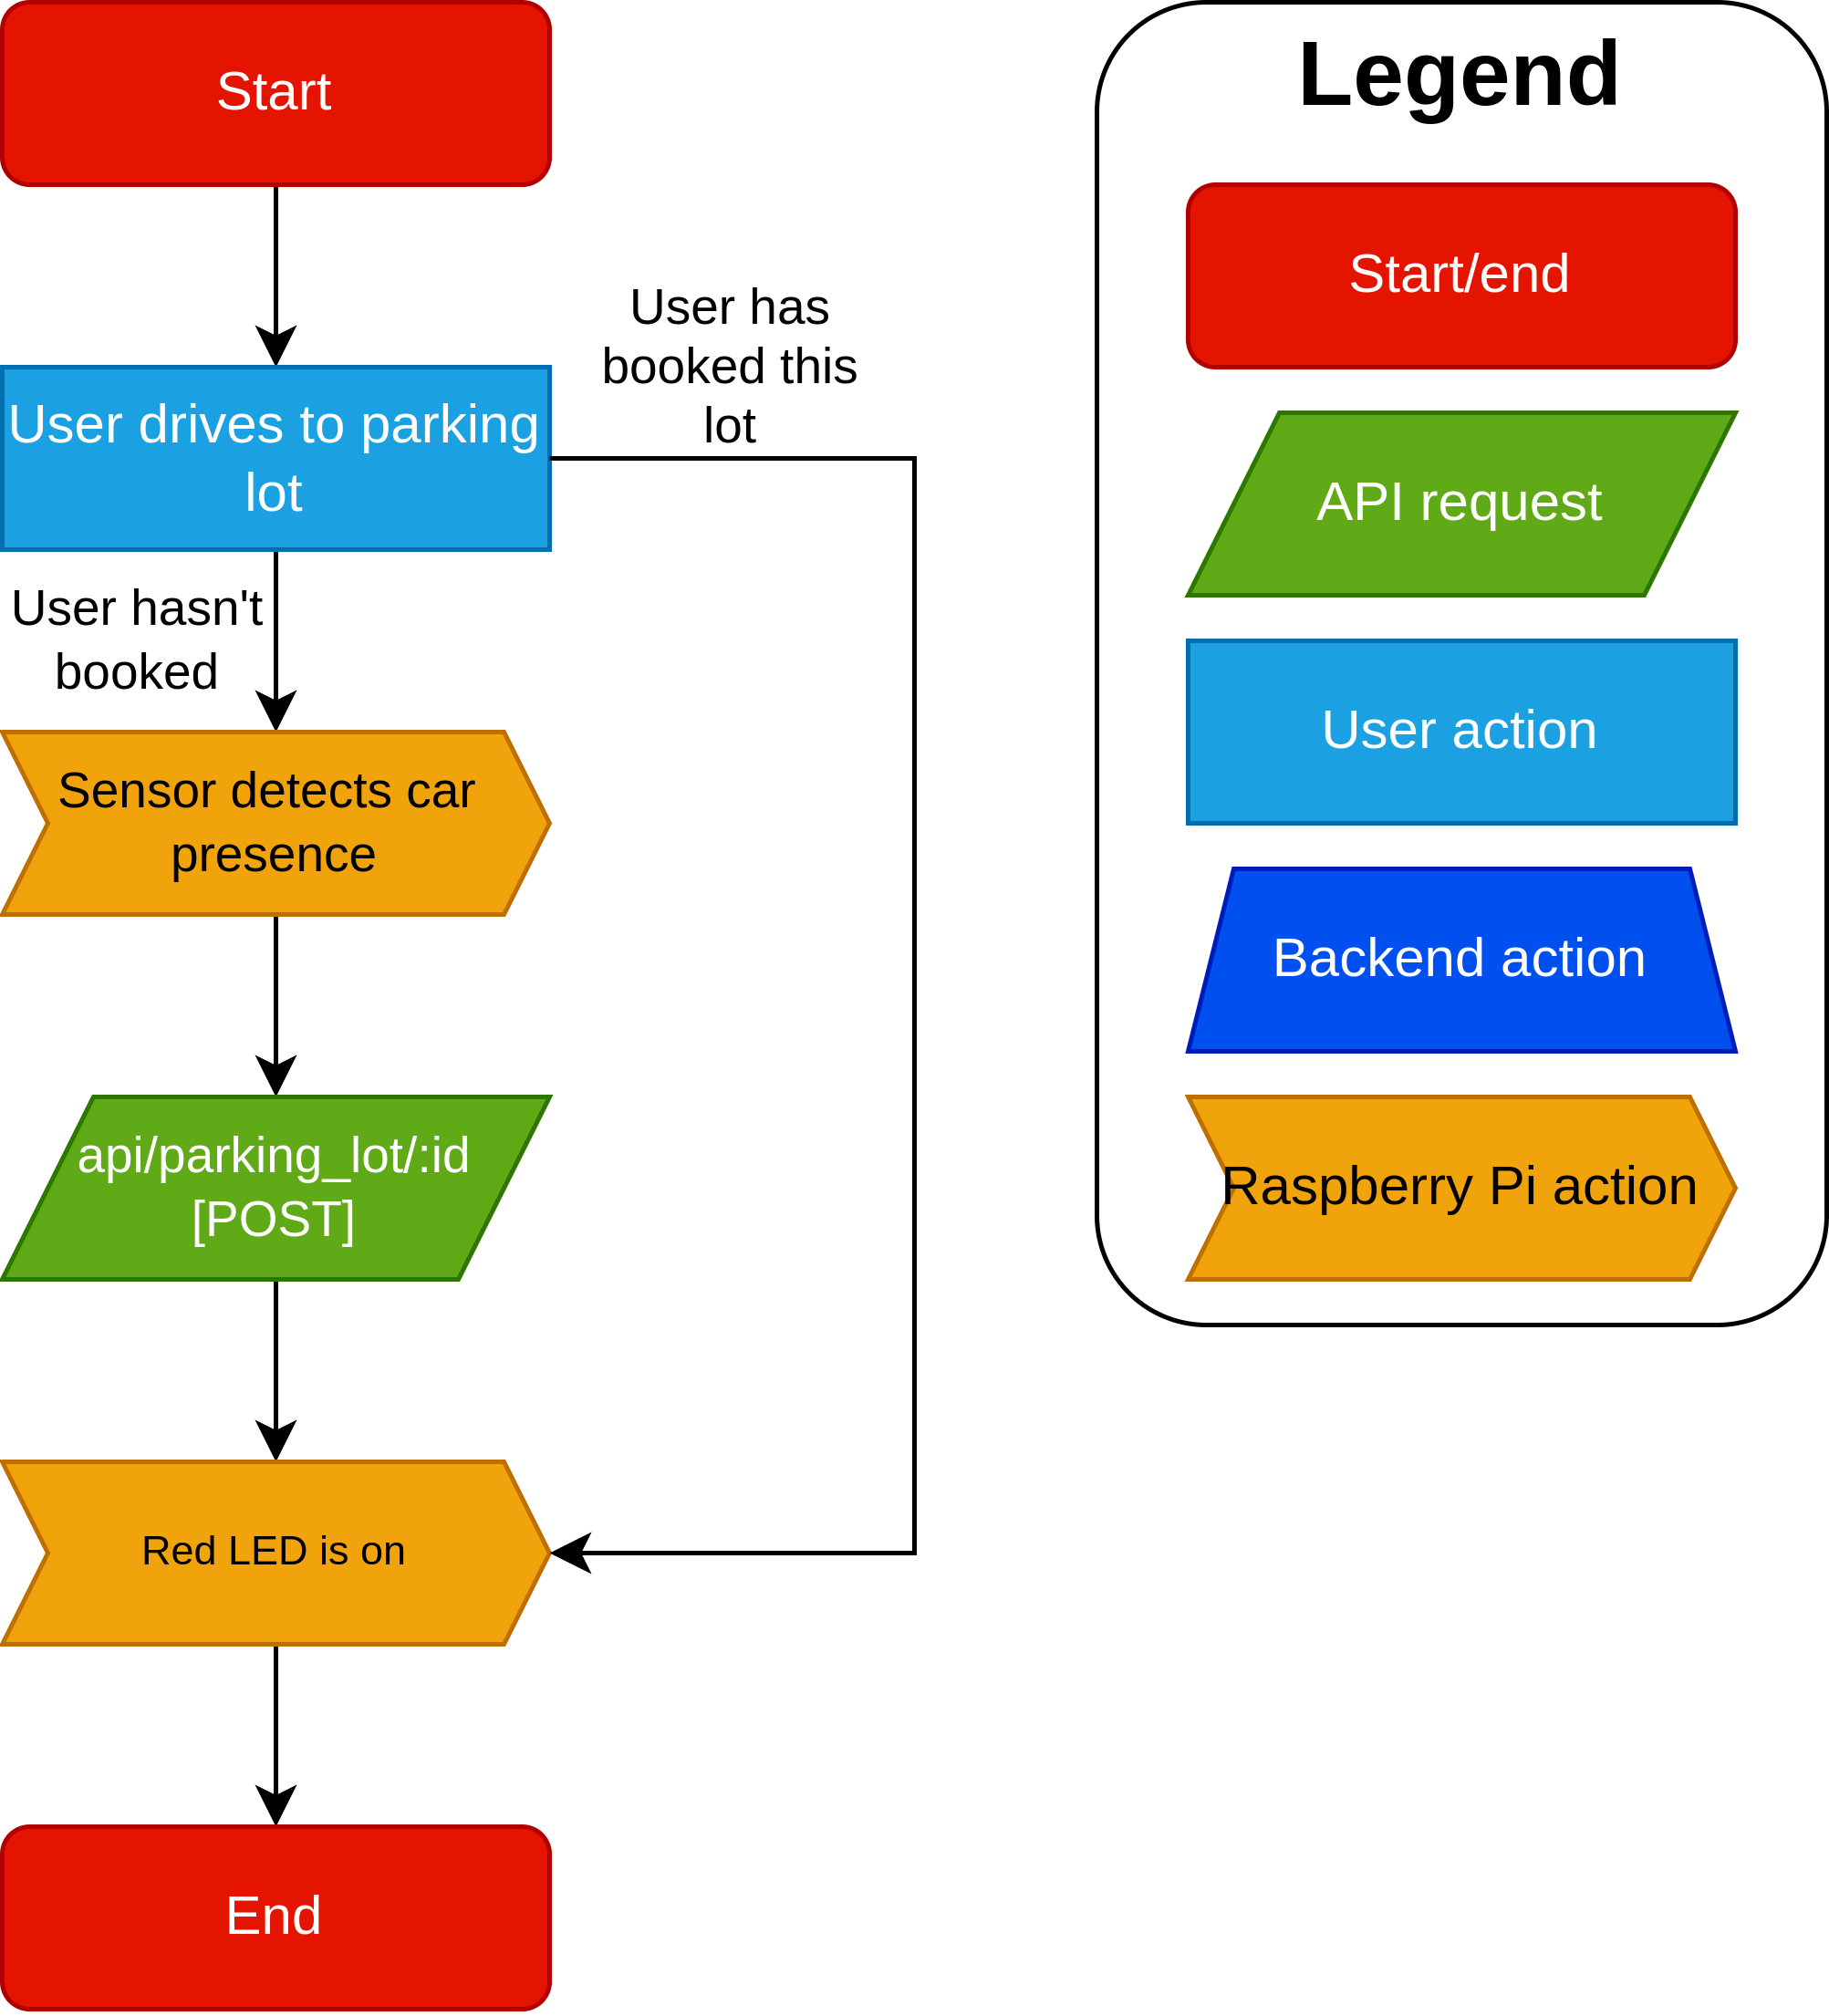
\includegraphics[width=7cm]{images/car_detection.drawio.png}
    \caption{Flowchart of the car detection process of the garage in both hardware, software and user terms.}
    \label{fig:car-detection}
\end{figure}

\begin{figure}[htp]
    \centering
    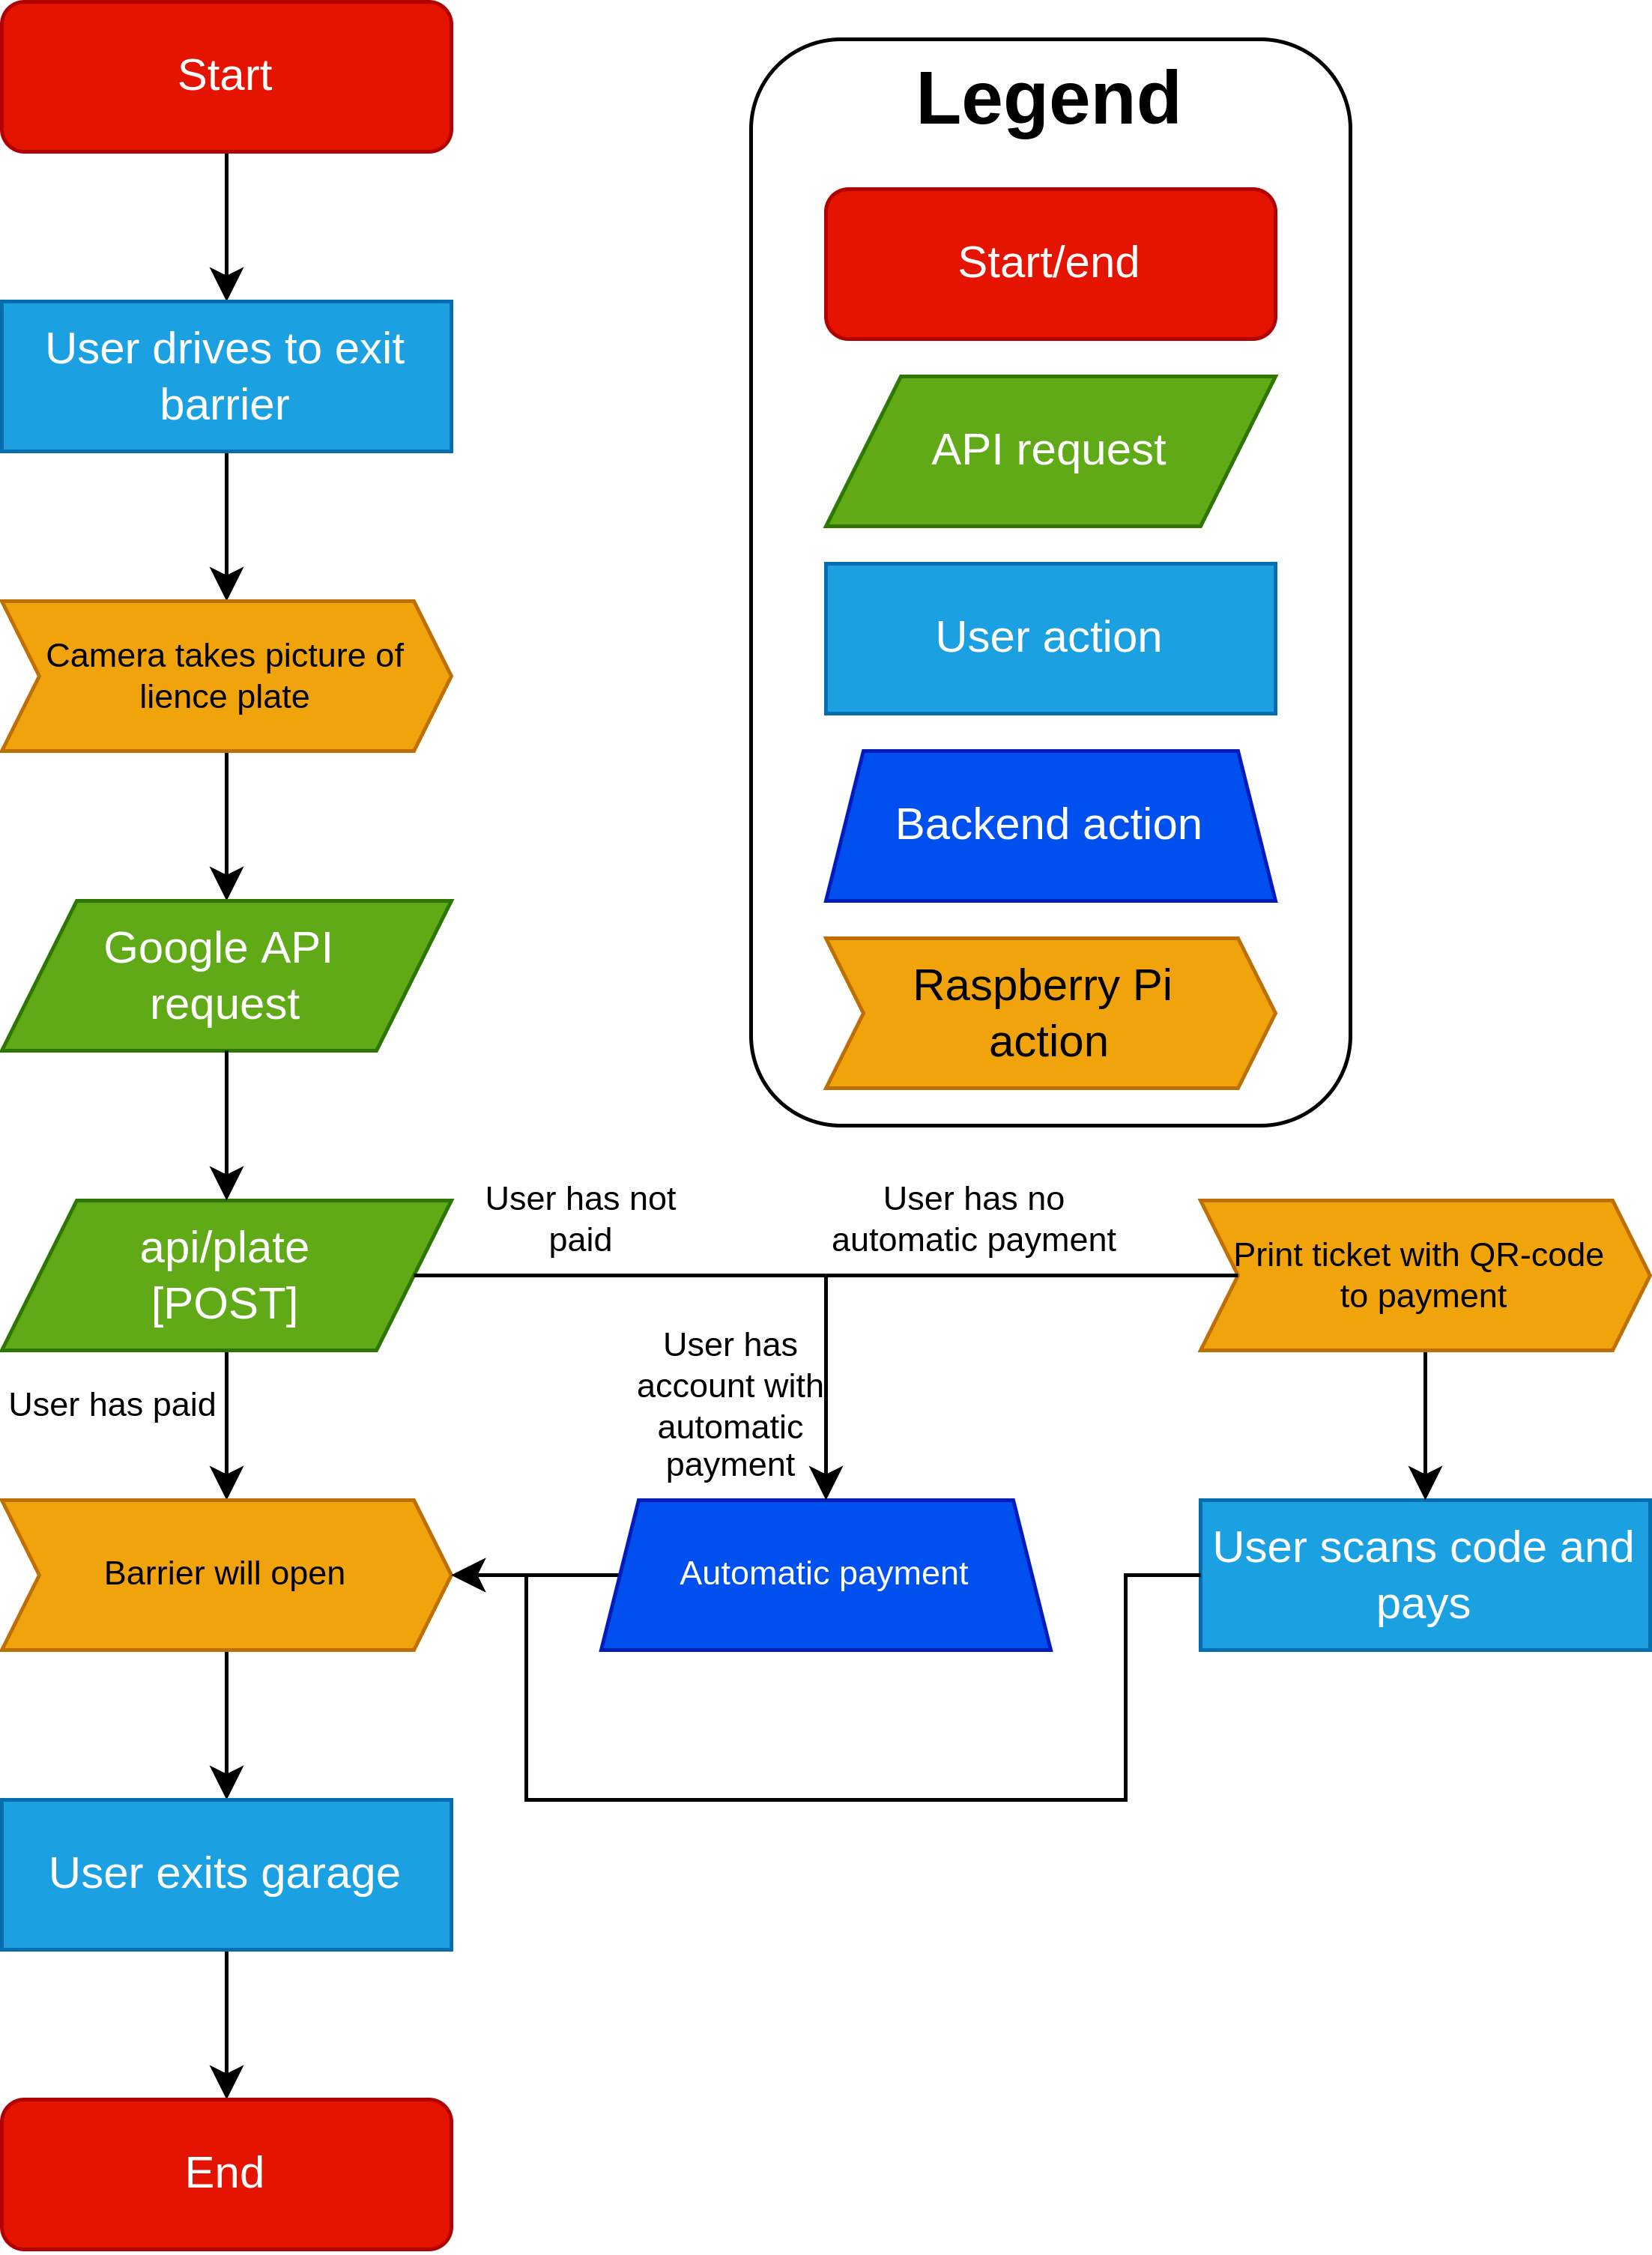
\includegraphics[width=8cm]{images/garage_exit.drawio.png}
    \caption{Flowchart of the exiting process of the garage in both hardware, software and user terms.}
    \label{fig:garage-exit}
\end{figure}

\section{Sequence diagrams}\label{app:sequence-diagrams}
\begin{figure}
    \centering
    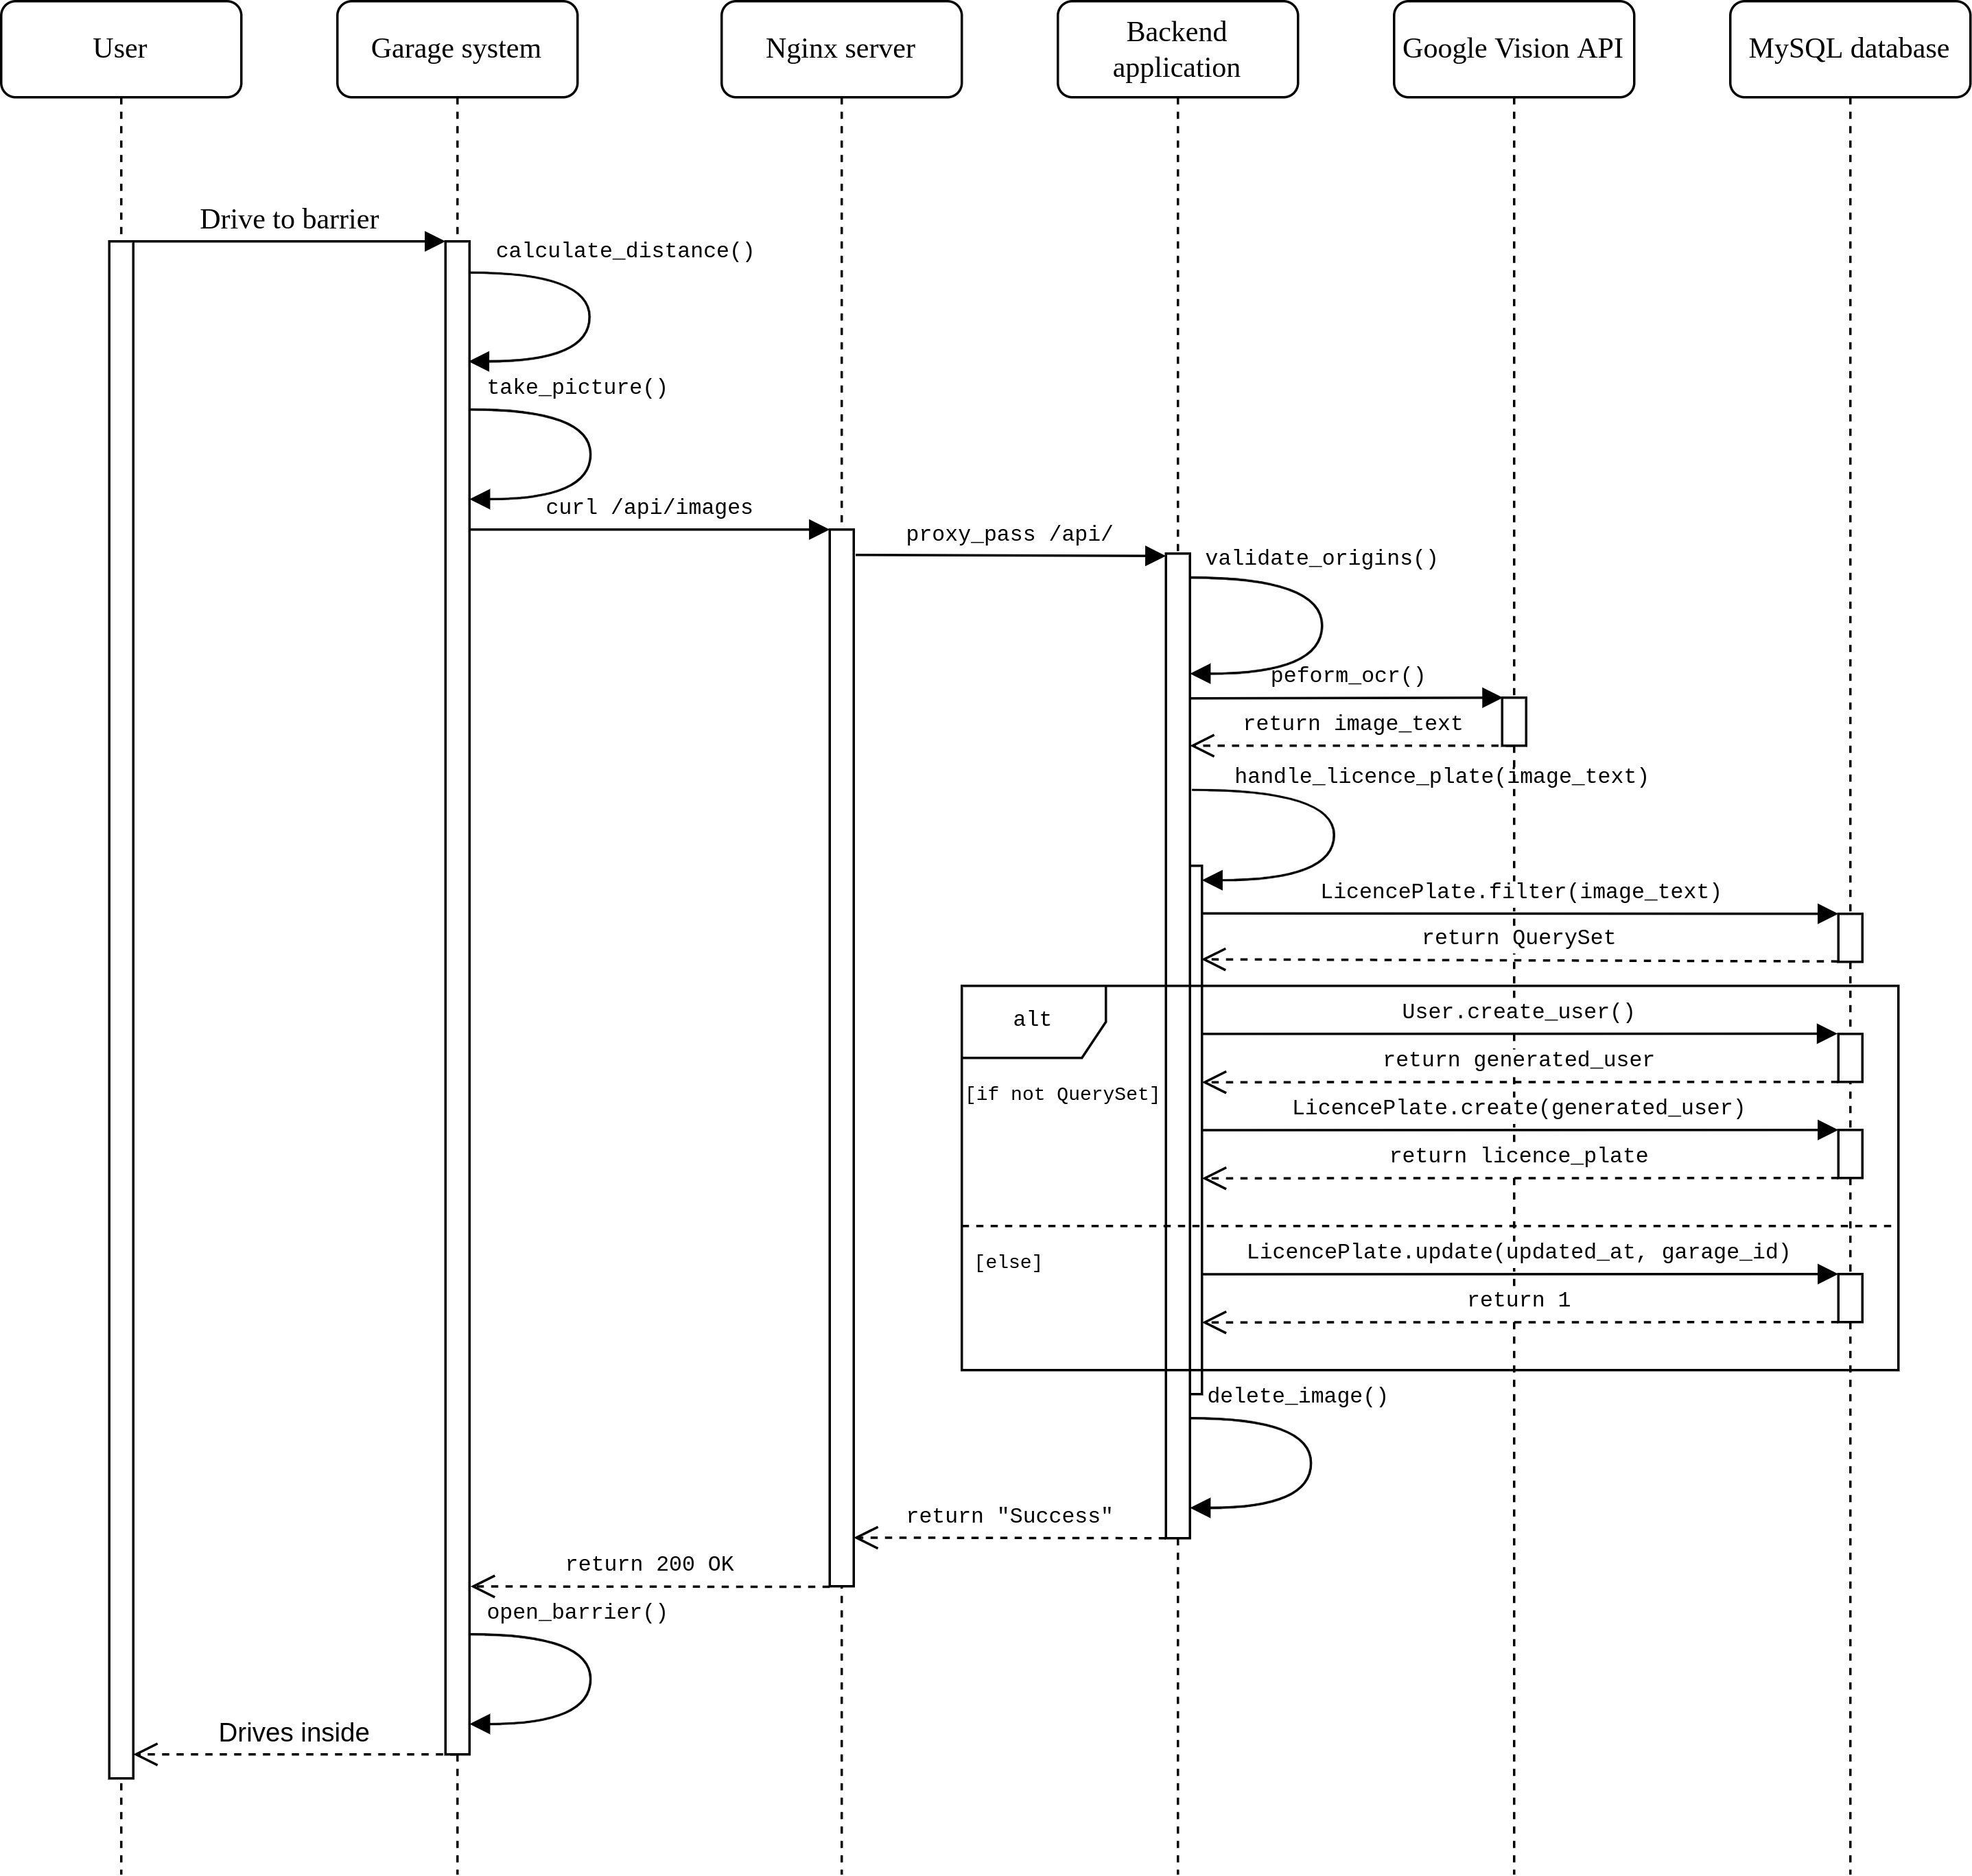
\includegraphics[width=16cm]{images/sequence_diagram_licence_plate.drawio.png}
    \caption{Sequence diagram of the licence plate registration in the local garage system.}
    \label{fig:sequence-diagram-licence-plate}
\end{figure}

\begin{figure}
    \centering
    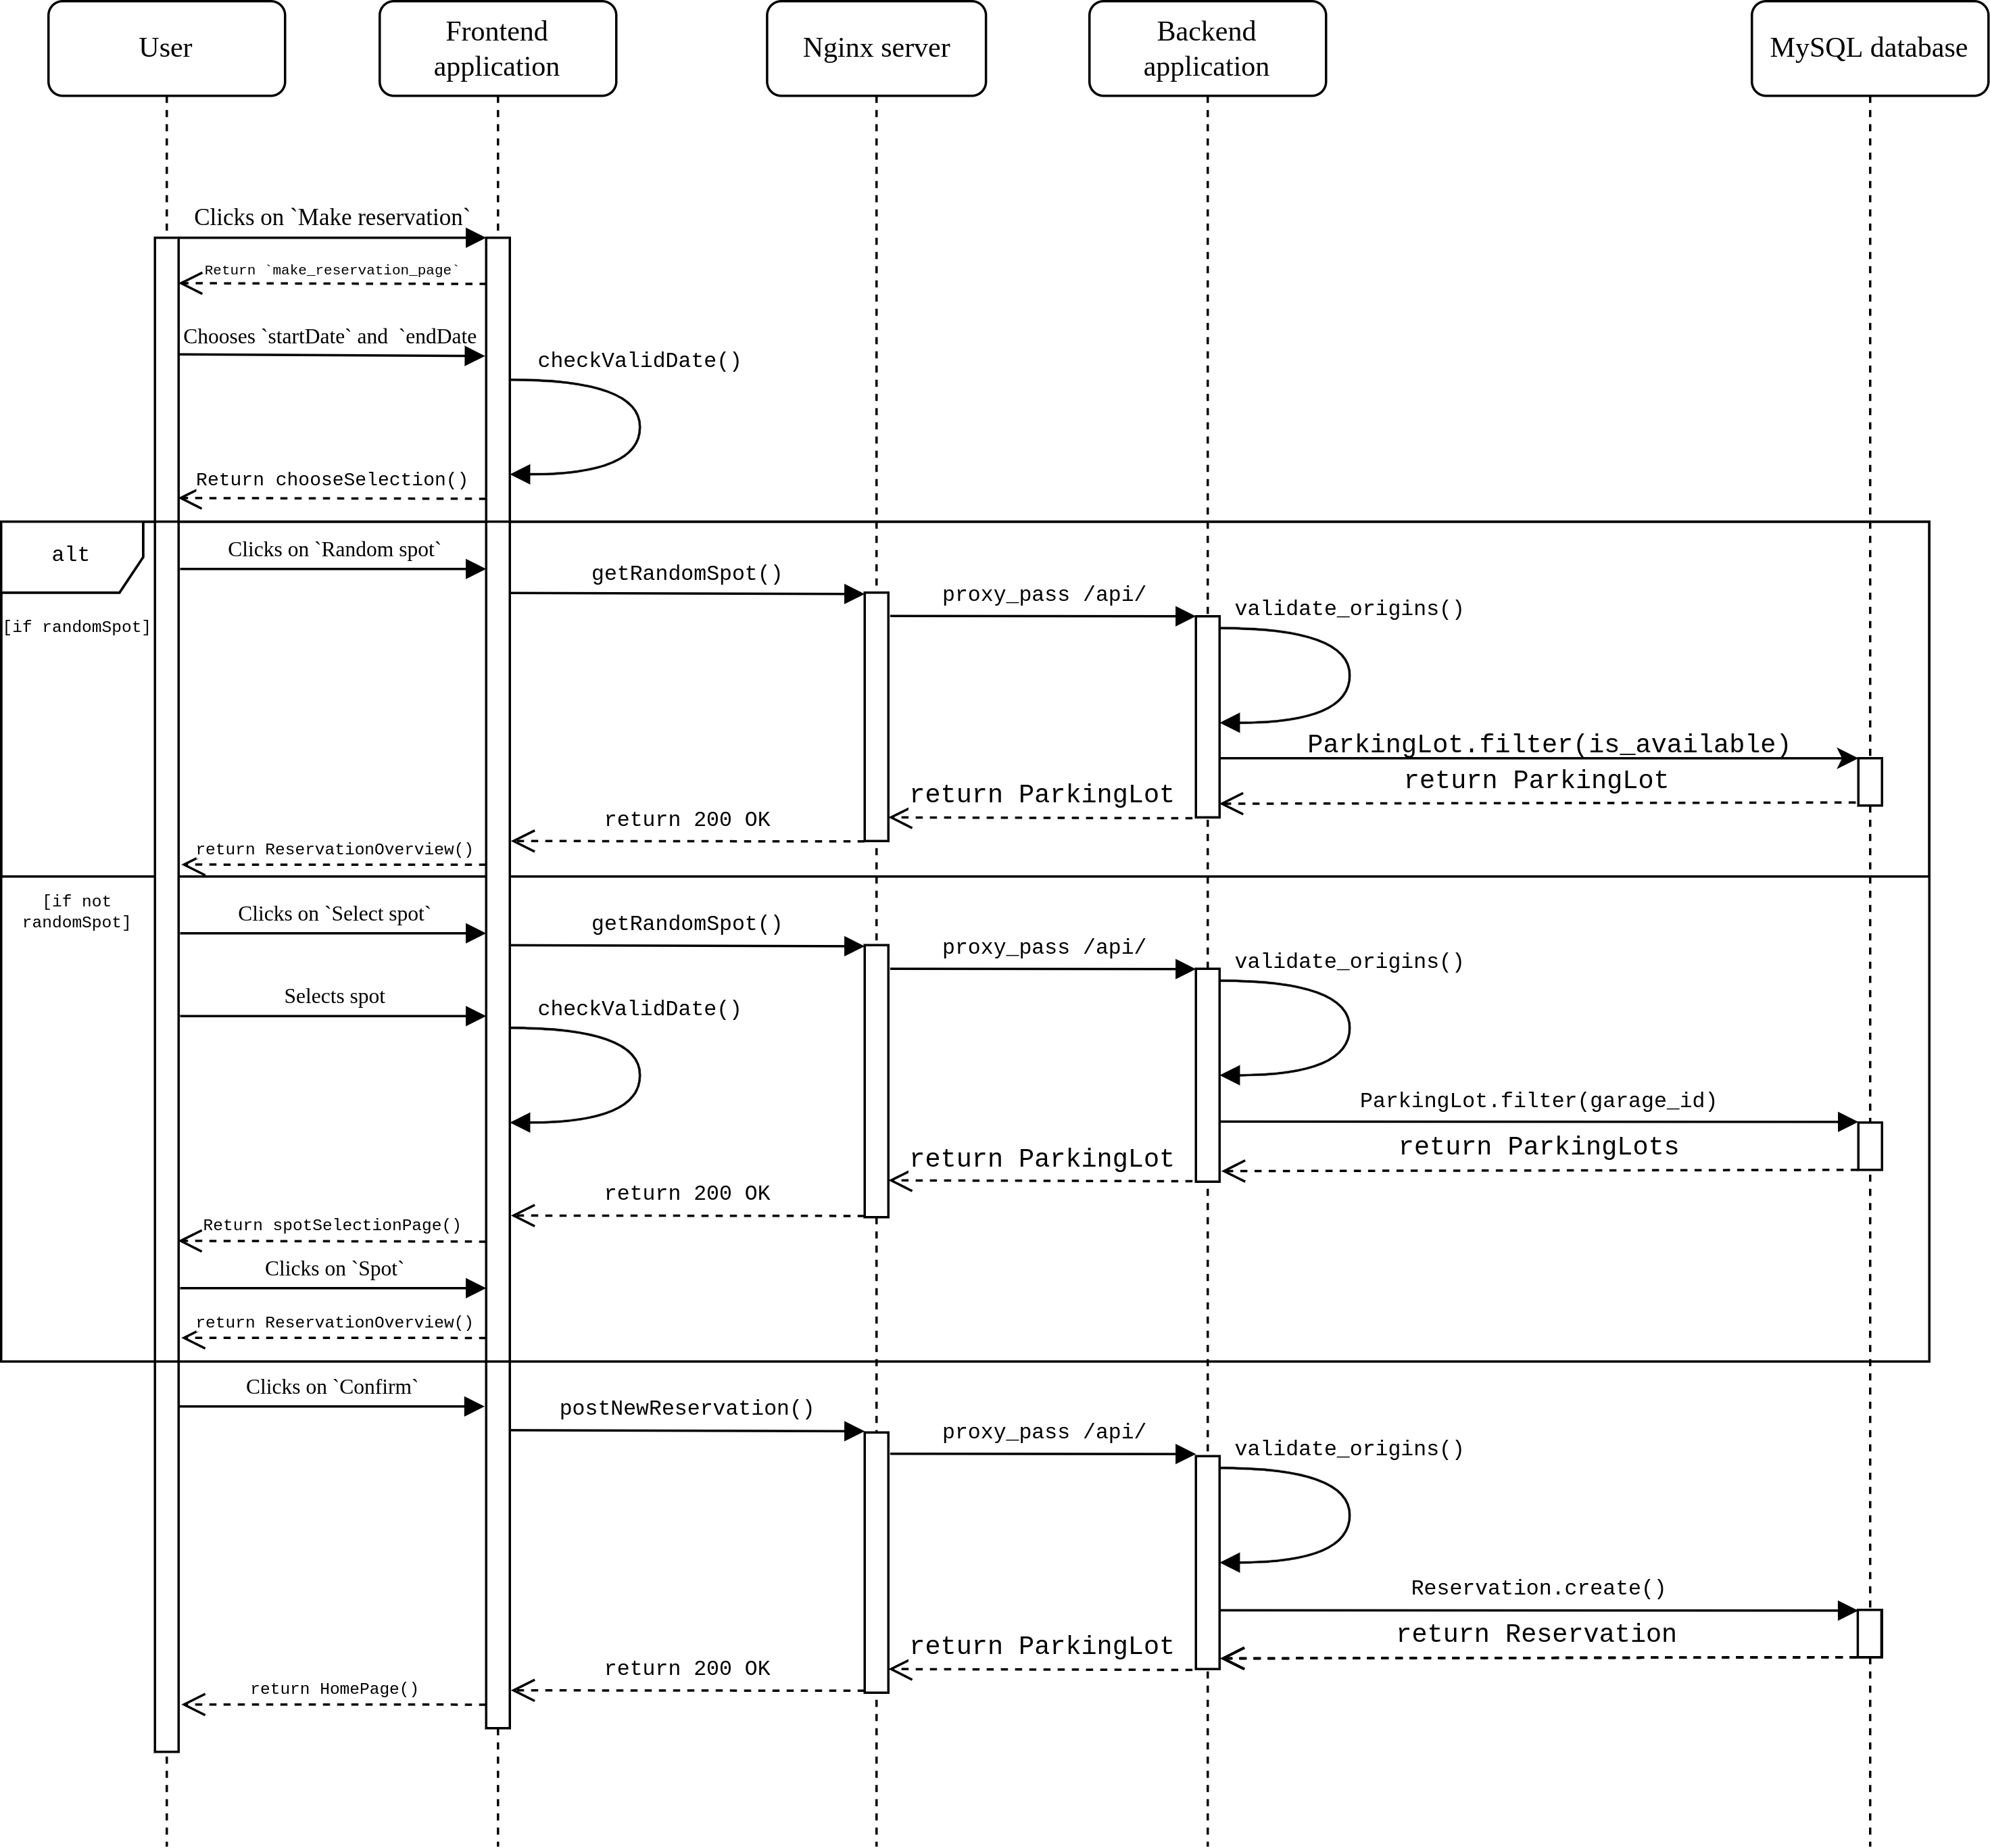
\includegraphics[width=16cm]{images/sequence_diagram_reservation.drawio.png}
    \caption{Sequence diagram of the reservation flow.}
    \label{fig:sequence-diagram-reservation}
\end{figure}

\end{appendices}


\end{document}
